\section{Unilateral effects with differentiated products: diversion, pricing pressure and pass-through}\label{sec:11-upp}

The homogeneous-goods analysis of \cref{sec:11-cournot} ties the price effect of a merger to market shares and to
the cost savings the merger creates. When products are differentiated, shares are a poor guide. Two firms with
small shares can be each other's closest substitutes. Two large firms can sell products that few consumers regard
as alternatives. The economics of a differentiated-products merger runs through a single object: the fraction of
the sales that one merging product loses after a price increase that the other merging product captures.

This section develops that idea in four steps. We first show that a merger of Bertrand competitors raises all
prices and is profitable in a standard linear model, in contrast with the Cournot merger paradox. We then define
diversion ratios and derive them for the logit, nested logit and random coefficients models. Next we derive the
upward pricing pressure test of \citet{FarrellShapiro2010} with its refinements. Finally we show that turning
pricing pressure into a predicted price change requires the pass-through rate, which depends on the curvature of
demand. \Cref{sec:11-simulation} then computes full post-merger equilibria.

We keep the global notation and add a few symbols. The merging products are 1 and 2. When we follow
\citet{FarrellShapiro2010} we also call their owners firms A and B. Quantities are $q_j(p)$ and marginal costs
$c_j$, which we take to be constant. This $c_j$ is the $mc_j$ of \cref{ch:diffprod}. We return to $mc_j$ in the
matrix formulas of \cref{sec:11-simulation,sec:11-millercoors}, which follow \cref{ch:diffprod}. The \emph{Lerner margin} of product $j$ is $L_j = \frac{p_j - c_j}{p_j}$.
Farrell and Shapiro write $M$ for it, but $M_t$ denotes market size in this book. The \emph{markup over cost} is
$\bar m_j = \frac{p_j - c_j}{c_j}$, and the two are linked by $\frac{1 - L_j}{L_j} = \frac{c_j}{p_j - c_j} =
\frac{1}{\bar m_j}$. A merger may lower marginal cost by the fraction $E_j$ of $c_j$. Pass-through is
$\rho = \frac{dp}{dc}$, which Farrell and Shapiro write as $R$. The curvature of a demand curve is measured by
$\psi = \frac{p\,q''(p)}{q'(p)}$. Ownership matrices before and after a merger are $\Omega^{pre}$ and
$\Omega^{post}$, and $\Delta$ is the matrix of share derivatives with $(j,k)$ element
$\frac{\partial s_j}{\partial p_k}$.

\subsection{Mergers of Bertrand competitors}\label{sec:11-dd}

\citet{DeneckereDavidson1985} showed that price competition overturns the merger paradox of
\cref{sec:11-cournot}. Under Cournot competition, quantities are strategic substitutes. Outsiders expand output when
the merged firm contracts, and a merger without synergies is often unprofitable. Under Bertrand competition with
differentiated products, prices are \emph{strategic complements}: a firm's best price rises with its rivals'
prices. Outsiders respond to the merged firm's higher prices by raising their own prices, and this response makes
the merger more profitable. We work out a linear example in closed form because later sections reuse it.

\begin{assumption}[Symmetric linear Bertrand oligopoly]\label{ass:11-linear}
There are $N \ge 3$ single-product firms with constant marginal cost $c$. Demand for product $j$ is
\begin{equation}\label{eq:11-lin-demand}
  q_j = a - b\,p_j + d \sum_{k \ne j} p_k , \qquad b > (N-1)d > 0 ,
\end{equation}
with $a > [b - (N-1)d]\,c$. Firms 1 and 2 merge without efficiencies. Firms set prices simultaneously before and
after the merger, and the merged firm maximizes the sum of the two products' profits.
\end{assumption}

The condition $b > (N-1)d$ says that a uniform increase in all prices lowers each firm's sales. It is convenient to
work with markups $m_j = p_j - c$. Substituting $p_k = c + m_k$ into \eqref{eq:11-lin-demand} gives
\begin{equation*}
  q_j = A - b\,m_j + d \sum_{k \ne j} m_k , \qquad A \equiv a - [b - (N-1)d]\,c > 0 .
\end{equation*}

Before the merger, firm $j$ maximizes $m_j q_j$. The first-order condition is $q_j - b\,m_j = 0$. In the symmetric
equilibrium all markups equal $m^0$, so
\begin{equation*}
  A - b\,m^0 + (N-1)d\,m^0 - b\,m^0 = 0
  \quad\Longrightarrow\quad
  m^0 = \frac{A}{2b - (N-1)d} .
\end{equation*}
Each firm sells $q^0 = b\,m^0$ and earns $\pi^0 = b\,(m^0)^2$.

After the merger, the merged firm maximizes $m_1 q_1 + m_2 q_2$. The derivative with respect to $m_1$ is
$q_1 - b\,m_1 + d\,m_2$, because a higher $m_1$ raises $q_2$ at the rate $d$. Outsiders keep the condition
$q_j - b\,m_j = 0$. We look for an equilibrium in which the two merging products share the markup $m_I$ and the
$N - 2$ outsiders share the markup $m_O$. Substituting the demand functions, the insiders' condition becomes
\begin{equation}\label{eq:11-dd-brI}
  A - 2(b - d)\,m_I + (N-2)d\,m_O = 0
  \quad\Longleftrightarrow\quad
  2(b-d)\,m_I = A + (N-2)d\,m_O ,
\end{equation}
and the outsiders' condition becomes
\begin{equation}\label{eq:11-dd-brO}
  A + 2d\,m_I + (N-3)d\,m_O - 2b\,m_O = 0
  \quad\Longleftrightarrow\quad
  \beta\, m_O = A + 2d\,m_I , \qquad \beta \equiv 2b - (N-3)d .
\end{equation}
Both are upward-sloping best-response relations, the signature of strategic complements. The pre-merger markup
also satisfies \eqref{eq:11-dd-brO} with $m_I = m_O = m^0$, since $\beta m^0 - 2d\,m^0 = [2b - (N-1)d]\,m^0 = A$.
Subtracting this identity from \eqref{eq:11-dd-brO} gives
\begin{equation}\label{eq:11-dd-ratio}
  m_O - m^0 = \frac{2d}{2b - (N-3)d}\,\big(m_I - m^0\big) .
\end{equation}

To solve for $m_I$, substitute $m_O$ from \eqref{eq:11-dd-brO} into \eqref{eq:11-dd-brI} and multiply by $\beta$:
\begin{equation*}
  \big[2(b-d)\beta - 2(N-2)d^2\big]\, m_I = A\beta + (N-2)d\,A = A\,(2b + d) .
\end{equation*}
Expanding the bracket gives $2\Gamma$ with $\Gamma \equiv 2b^2 - (N-1)bd - d^2$, so
\begin{equation*}
  m_I = \frac{A\,(2b + d)}{2\Gamma} .
\end{equation*}
The constant $\Gamma$, unrelated to the function $\Gamma_n$ in the proof of \cref{prop:11-synergy}, is positive: $b > (N-1)d$ implies $2b - (N-1)d > b$, so $b[2b - (N-1)d] > b^2 > d^2$.
Subtracting $m^0$ and simplifying the numerator, $(2b+d)[2b - (N-1)d] - 2\Gamma = d\beta$, so
\begin{equation}\label{eq:11-dd-increase}
  m_I - m^0 = \frac{A\,d\,\beta}{2\Gamma\,[2b - (N-1)d]} > 0 ,
  \qquad
  m_O - m^0 = \frac{A\,d^2}{\Gamma\,[2b - (N-1)d]} > 0 .
\end{equation}
With three firms, $\beta = 2b$ and the formulas reduce to $m_I = \frac{A(2b+d)}{2(2b^2 - 2bd - d^2)}$ and
$m_O = \frac{A\,b}{2b^2 - 2bd - d^2}$.

\begin{proposition}[Bertrand mergers]\label{prop:11-dd}
Under \cref{ass:11-linear}:
\begin{enumerate}[label=(\roman*)]
  \item the merger raises the prices of all products, and the merging firms' prices rise the most,
  \item each outsider's price rises by the fraction $\frac{2d}{2b - (N-3)d} \in (0,1)$ of the merging firms'
        price increase,
  \item the merger is profitable for the merging firms,
  \item every outsider's profit rises. With $N = 3$, the outsider gains more than each merging firm.
\end{enumerate}
\end{proposition}

\begin{proof}
Parts (i) and (ii) follow from \eqref{eq:11-dd-ratio} and \eqref{eq:11-dd-increase}. The fraction in (ii) is below
one because $2b - (N-3)d > 2(N-1)d - (N-3)d = (N+1)d > 2d$. For (iii), the merged firm could keep both markups at
$m^0$. Since outsiders now charge $m_O > m^0$ and $d > 0$, each merging product would then sell more than $q^0$ at the
markup $m^0$, so joint profit would exceed $2\pi^0$. The merged firm's optimal markups earn at least this much. For
(iv), the outsider's first-order condition gives $q_O = b\,m_O$, so its profit is $b\,m_O^2 > b\,(m^0)^2 = \pi^0$.
With $N = 3$, the insiders' condition gives $q_I = (b - d)m_I$, so each insider earns $(b - d)m_I^2$. Using the
three-firm formulas,
\begin{equation*}
  \frac{b\,m_O^2}{(b-d)\,m_I^2} = \frac{4b^3}{(b-d)(2b+d)^2} = \frac{4b^3}{4b^3 - 3bd^2 - d^3} > 1 .
\end{equation*}
\end{proof}

The profitability argument in (iii) does not depend on linearity. It uses only two facts: each merging product's
demand rises with outsiders' prices, and outsiders raise their prices after the merger. Both hold whenever goods are
substitutes and prices are strategic complements. A merger of price-setting firms therefore benefits the merging
parties even without synergies, and it benefits outsiders as well. Consumers bear the cost.

For a numerical illustration take $N = 3$, $A = 1$, $b = 1$ and $d = 0.25$. The
pre-merger markup is $m^0 = 0.6667$. After the merger the insiders' markup is $0.7826$, a rise of 17.4 percent, and
the outsider's markup is $0.6957$, a rise of 4.3 percent. The outsider's markup rises by $\frac{d}{b} = 0.25$ times
the insiders' increase, as \eqref{eq:11-dd-ratio} predicts. Profit per firm is $0.4444$ before the merger. It rises
to $0.4594$ for each insider (3.4 percent) and to $0.4839$ for the outsider (8.9 percent). The outsider free-rides on
the merged firm's restraint. \Cref{fig:11-ddbr} shows the equilibrium in the space of the two markups.

\begin{figure}[htbp]
\centering
\begin{tikzpicture}
\begin{axis}[
  width=0.72\textwidth, height=0.5\textwidth,
  xmin=0.60, xmax=0.84, ymin=0.60, ymax=0.75,
  xlabel={markup of each merging firm, $m_I$},
  ylabel={markup of the outsider, $m_O$},
  xtick={0.60,0.65,0.70,0.75,0.80},
  ytick={0.60,0.65,0.70,0.75},
  tick label style={font=\footnotesize},
  label style={font=\small},
  axis lines=left,
  clip=true,
]
\addplot[domain=0.60:0.84, samples=2, thick, color={rgb,255:red,235;green,104;blue,52}]
  {0.5 + 0.25*x} node[pos=0.93, above, font=\footnotesize, black] {outsider};
\addplot[domain=0.6571:0.6786, samples=2, thick, dashed, color={rgb,255:red,42;green,120;blue,214}]
  {7*x - 4};
\addplot[domain=0.7667:0.7917, samples=2, thick, color={rgb,255:red,42;green,120;blue,214}]
  {6*x - 4};
\node[font=\footnotesize, anchor=east] at (axis cs:0.673,0.738) {insiders, before};
\node[font=\footnotesize, anchor=east] at (axis cs:0.786,0.738) {insiders, after};
\addplot[only marks, mark=*, mark size=1.8pt] coordinates {(0.6667,0.6667) (0.7826,0.6957)};
\node[font=\footnotesize, anchor=north west] at (axis cs:0.6667,0.6667) {$(m^0, m^0)$};
\node[font=\footnotesize, anchor=north west] at (axis cs:0.7826,0.6957) {$(m_I, m_O)$};
\draw[-{Stealth[length=2mm]}, thin] (axis cs:0.684,0.62) -- (axis cs:0.762,0.62);
\node[font=\footnotesize, anchor=south] at (axis cs:0.723,0.62) {merger};
\end{axis}
\end{tikzpicture}
\caption{Best responses in the linear Bertrand example with $N = 3$, $A = 1$, $b = 1$ and $d = 0.25$. The
insiders' symmetric best response is $m_I = \frac{1 + 0.25\,m_O}{1.75}$ before the merger and
$m_I = \frac{1 + 0.25\,m_O}{1.5}$ after it. The outsider's best response is $m_O = \frac{1 + 0.5\,m_I}{2}$. The merger
shifts the insiders' curve to the right, and the outsider moves up along its own upward-sloping curve.}
\label{fig:11-ddbr}
\end{figure}

Part (ii) matters for retrospective studies. A rival's price is a tempting control for the merging firms' price, but
the rival's price also rises after the merger. \Cref{sec:11-retro} uses \eqref{eq:11-dd-ratio} to sign the resulting
bias of difference-in-differences estimates.

\subsection{Diversion ratios}\label{sec:11-diversion}

The price effect of a differentiated-products merger depends on how closely the merging products compete. The
diversion ratio, which \cref{sec:11-critloss} used to resolve the critical loss paradox, measures this closeness
directly. Recall from \cref{def:04-diversion} that the diversion ratio from product $j$ to product $k \ne j$ is
\begin{equation*}
  D_{jk} = -\dfrac{\frac{\partial q_k(p)}{\partial p_j}}{\frac{\partial q_j(p)}{\partial p_j}} ,
\end{equation*}
the fraction of $j$'s lost sales that $k$ captures when $p_j$ rises. \Cref{sec:04-diversion}
derived its basic properties. With an outside good, the diversion ratios from $j$ to all other options sum to one
(\cref{prop:04-diversion-adding}). In elasticity form, $D_{jk} = \frac{\varepsilon_{kj}\,q_k}{\varepsilon_j\,q_j}$ by
\eqref{eq:04-diversion-elast}. Diversion is directional. In general $D_{jk} \ne D_{kj}$, and the two enter the merger
analysis separately. Merger analysis also needs the diversion from one product to a group of products.

\begin{definition}[Aggregate diversion to a set]\label{def:11-aggdiv}
The \emph{aggregate diversion ratio} of product $j$ to a set of products $\mathcal{K}$ with $j \notin \mathcal{K}$ is
$\bar D_j(\mathcal{K}) = \sum_{k \in \mathcal{K}} D_{jk}$. We drop the argument when the set is clear from the context.
\end{definition}

The set $\mathcal{K}$ can be a candidate market, as in \cref{prop:11-aggdiv}. It can also be the products of the
merger partner, as in \eqref{eq:11-upp-multi}, or a group of equally close substitutes, as in
\eqref{eq:11-share-proxy}. When $\mathcal{K}$ contains every inside good other than $j$, \cref{prop:04-diversion-adding}
gives $\bar D_j(\mathcal{K}) = 1 - D_{j0}$, where $D_{j0}$ is the diversion to the outside good. The rest of this
subsection recalls the diversion ratios of the main demand models from \cref{sec:04-diversion-systems} and adds what
matters for mergers.

\casehead{Logit} With logit demand (\cref{ch:logit}), the share derivatives are
$\frac{\partial s_j}{\partial p_j} = -\alpha s_j (1 - s_j)$ and $\frac{\partial s_k}{\partial p_j} = \alpha s_j s_k$
for $k \ne j$. Their ratio gives \eqref{eq:04-diversion-logit},
\begin{equation}\label{eq:11-logit-diversion}
  D_{jk} = \frac{\alpha s_j s_k}{\alpha s_j (1 - s_j)} = \frac{s_k}{1 - s_j} .
\end{equation}
Diversion is proportional to the share of the receiving product. This is the independence of irrelevant
alternatives at work: product $j$'s lost customers spread over the other goods, including the outside good, in
proportion to their shares. The logit therefore assumes that all products are equally close substitutes for $j$.
This assumption is the formal justification for share-based merger analysis \citep{Willig1991}. Directionality is
visible in \eqref{eq:11-logit-diversion}. With $s_1 = 0.4$ and $s_2 = 0.1$, $D_{12} = \frac{0.1}{0.6} = 0.17$ while
$D_{21} = \frac{0.4}{0.9} = 0.44$.

\casehead{Nested logit} Partition the inside goods into nests $g$ with nesting parameter $\sigma \in [0,1)$
(\cref{ch:logit}). Let $H_g = \sum_{k \in g} e^{\frac{\delta_k}{1 - \sigma}}$. The within-nest share, the nest share
and the market share are
\begin{equation*}
  s_{j|g} = \frac{e^{\frac{\delta_j}{1-\sigma}}}{H_g} , \qquad
  s_g = \frac{H_g^{1-\sigma}}{1 + \sum_h H_h^{1-\sigma}} , \qquad
  s_j = s_{j|g}\, s_g .
\end{equation*}
Taking logs, $\ln s_j = \frac{\delta_j}{1-\sigma} - \sigma \ln H_g - \ln\big(1 + \sum_h H_h^{1-\sigma}\big)$. Since
$\frac{\partial \ln H_g}{\partial \delta_j} = \frac{s_{j|g}}{1 - \sigma}$ for $j \in g$ and
$\frac{\partial}{\partial \delta_j}\ln\big(1 + \sum_h H_h^{1-\sigma}\big) = s_j$, we get
\begin{equation*}
  \frac{\partial \ln s_j}{\partial \delta_j} = \frac{1 - \sigma s_{j|g}}{1-\sigma} - s_j , \qquad
  \frac{\partial \ln s_k}{\partial \delta_j} =
  \begin{cases}
    -\frac{\sigma s_{j|g}}{1-\sigma} - s_j & \text{if } k \in g, \\[2pt]
    -s_j & \text{if } k \notin g .
  \end{cases}
\end{equation*}
Multiplying by $-\alpha s_k$ gives the price derivatives. Dividing and using $s_k s_{j|g} = s_j s_{k|g}$ for products
in the same nest,
\begin{equation}\label{eq:11-nl-diversion}
  D_{jk} =
  \begin{cases}
    \dfrac{\sigma s_{k|g} + (1-\sigma) s_k}{1 - \sigma s_{j|g} - (1-\sigma) s_j} & \text{if } k \text{ is in } j\text{'s nest } g, \\[12pt]
    \dfrac{(1-\sigma) s_k}{1 - \sigma s_{j|g} - (1-\sigma) s_j} & \text{otherwise.}
  \end{cases}
\end{equation}
This is \eqref{eq:04-diversion-nl}. We derive it here because \cref{sec:11-bv} reuses the intermediate steps. At
$\sigma = 0$ both cases reduce to the logit formula. As $\sigma \to 1$, diversion to the other nests vanishes and
diversion within the nest approaches $\frac{s_{k|g}}{1 - s_{j|g}}$. The nested logit thus lets the analyst declare in
advance which products are close. The declaration is a modeling choice, and the estimated $\sigma$ disciplines only
its strength.

\casehead{Random coefficients} With random coefficients (\cref{ch:blp}), consumer $i$ has price coefficient
$\alpha_i$ and logit choice probabilities $s_{ij}$, and $s_j = \int s_{ij}\,dP(i)$. Differentiating under the integral
gives \eqref{eq:04-diversion-marginal}. The market-level ratio $D_{jk}$ is a weighted average of the individual logit
ratios $\frac{s_{ik}}{1 - s_{ij}}$, with weights proportional to $\alpha_i s_{ij}(1 - s_{ij})$. The weights are each
consumer's contribution to $j$'s lost sales, so they favor price-sensitive consumers who are likely to buy $j$. Those consumers'
second choices resemble $j$ in characteristics, which is how the model generates diversion toward similar products.
There is no closed form, and diversion is computed from the estimated Jacobian.

\casehead{Shares as a proxy} \citet[Section 2.G]{FarrellShapiro2010} note that diversion can be approximated from
shares when the products in some group are about equally close substitutes for product 1. If the aggregate
diversion from product 1 to the group is $\bar D_1$ and $s_k$ denotes shares within the group, then
\begin{equation}\label{eq:11-share-proxy}
  D_{12} \approx \bar D_1 \frac{s_2}{1 - s_1} .
\end{equation}
The group need not be an antitrust market, and product 1 need not belong to it. The conditions for this proxy, equal
closeness and a known aggregate diversion, differ from the criteria used to define markets. In a candidate market
that just passes a breakeven SSNIP of size $X$ with uniform margins, aggregate diversion equals $\frac{X}{X + L}$
(\cref{sec:11-marketdef}). Farrell and Shapiro's appendix combines this with \eqref{eq:11-share-proxy}, and the
resulting proxy for upward pricing pressure does not line up with concentration thresholds. The distribution of
sales among non-merging firms changes the HHI but not the proxy.

\casehead{Measurement} Diversion ratios can be estimated econometrically from a demand system. Firms also track
them in the ordinary course of business, to learn whom they lose customers to and whom they can win them from.
Consumer surveys and switching data are other sources. In bidding markets the diversion ratio from A to B is the
probability that B is the buyer's second choice when A wins, which win-loss records can reveal
\citep[Section 2.G]{FarrellShapiro2010}. In the Oracle and PeopleSoft merger, bid data showed that the two firms
were often the two leading bidders for large customers. These sources need not measure the same object. The
pricing conditions below use \emph{marginal} diversion, the response to a small change in $p_1$ near pre-merger
prices. Second-choice surveys, win-loss records and product removals such as stock-outs describe where buyers go
when product 1 is unavailable, which is a large change. With heterogeneous buyers the two ratios differ, because
they weight consumer types differently (\eqref{eq:04-diversion-marginal} and \eqref{eq:04-diversion-secondchoice}
in \cref{sec:04-diversion}). Take two equally common logit types with price coefficients 1 and 2. Over product 1,
product 2 and the outside good, their choice probabilities are $(0.8, 0.1, 0.1)$ and $(0.2, 0.7, 0.1)$. Marginal
diversion from 1 to 2 is then 0.75, while removing product 1 diverts only 0.575 of its buyers to product 2. Turning
such data into marginal diversion therefore requires a demand model or extra restrictions, such as a single logit
type. Diversion after a moderate price change, or after a change in $p_2$ instead of $p_1$, can differ again.

\subsection{Upward pricing pressure: Farrell and Shapiro (2010)}\label{sec:11-uppfs}

\casehead{The question} \citet{FarrellShapiro2010} ask how an antitrust agency can establish a simple, rebuttable
presumption that a merger of sellers of differentiated products will raise prices. The established presumption
defines a relevant market and computes the change in concentration. With differentiated products, market boundaries
are often arbitrary, and the closeness of the merging products matters more than their shares. Farrell and Shapiro
propose instead to ask whether the merger creates net upward pricing pressure (UPP). The test weighs the loss of
direct competition between the merging firms against the marginal-cost savings of the merger. It uses only
pre-merger margins and diversion ratios, and it does not require predicting the size of the price change. The idea
builds on \citet{Werden1996} and \citet{OBrienSalop2000}. It shaped the treatment of the ``value of diverted
sales'' in the 2010 Horizontal Merger Guidelines \citep{USDOJFTC2010}. We follow the version of 25 November 2008, and
equation and proposition numbers refer to it.

\casehead{The general idea} Think of the merged firm as running two divisions, A and B, that used to be separate
firms. Let $s$ be any variable that division A chooses to boost its sales, such as a price cut or advertising, and let
$x_1(s)$ be the sales of A's product, with $x_1'(s) > 0$. Before the merger, A maximizes $\pi_A(s)$. After the
merger, headquarters maximizes $\pi_A(s) + \pi_B(s)$. Compare this with a separate firm A that pays a per-unit tax $t$
on its product. Its objective $\pi_A(s) - t\,x_1(s)$ has first-order condition $\pi_A'(s) - t\,x_1'(s) = 0$. The
merged firm's condition is $\pi_A'(s) + \pi_B'(s) = 0$. The two coincide at a given $s$ when
\begin{equation}\label{eq:11-tax-general}
  t = -\frac{\pi_B'(s)}{x_1'(s)} .
\end{equation}
If A's actions hurt B, then $\pi_B'(s) < 0$ and the tax is positive. The merger acts on A's incentives like a tax on
its sales, and the tax involves only first derivatives. The change in $s$ itself would require second derivatives. If
A acquires a small share $\theta$ of B, the implicit function theorem applied to $\pi_A'(s) + \theta\pi_B'(s) = 0$
gives $\frac{ds}{d\theta} = -\frac{\pi_B'(s)}{\pi_A''(s)}$ at $\theta = 0$ \citep[fn.~22]{FarrellShapiro2010}. The
denominator depends on the curvature of A's residual demand and, in an oligopoly, on rivals' responses. Farrell and
Shapiro therefore build their test on the tax, which is easier to estimate.

\casehead{Bertrand pricing} Specialize to single-product Bertrand competitors. Firm A sells product 1 and firm B
sells product 2. Before the merger, A sets $p_1$ to maximize $(p_1 - c_1)q_1(p)$, which gives
\begin{equation}\label{eq:11-foc-pre}
  q_1 + (p_1 - c_1)\frac{\partial q_1}{\partial p_1} = 0 .
\end{equation}
After the merger, headquarters sets $p_1$ to maximize $(p_1 - c_1)q_1 + (p_2 - c_2)q_2$. The derivative of joint
profit with respect to $p_1$, evaluated at the pre-merger prices, is
\begin{equation*}
  \frac{\partial(\pi_A + \pi_B)}{\partial p_1}
  = \underbrace{q_1 + (p_1 - c_1)\frac{\partial q_1}{\partial p_1}}_{=\,0 \text{ by } \eqref{eq:11-foc-pre}}
    + (p_2 - c_2)\frac{\partial q_2}{\partial p_1}
  = (p_2 - c_2)\frac{\partial q_2}{\partial p_1} > 0 .
\end{equation*}
At pre-merger prices the merged firm wants to raise $p_1$. Dividing by $-\frac{\partial q_1}{\partial p_1} > 0$
converts the derivative into a per-unit amount,
\begin{equation}\label{eq:11-upp}
  \mathit{UPP}_1 = D_{12}\,(p_2 - c_2) .
\end{equation}
\Cref{sec:04-diversion-merger} previewed this calculation as the cannibalization term of \eqref{eq:04-upp}.

The same expression follows from \eqref{eq:11-tax-general}. A price cut that sells one more unit of product 1 takes
$D_{12}$ units from product 2, and each lost unit of product 2 costs B its margin $p_2 - c_2$. Hence
$-\frac{d\pi_B}{dq_1} = \frac{d\pi_B}{dq_2}\left|\frac{dq_2}{dq_1}\right| = (p_2 - c_2)D_{12}$. Farrell and Shapiro
call this the \emph{first-round tax} $t_1 = D_{12}(p_2 - c_2)$, and likewise $t_2 = D_{21}(p_1 - c_1)$. Dividing the
post-merger first-order condition for $p_1$ by $-\frac{\partial q_1}{\partial p_1}$ shows the tax interpretation at
any prices:
\begin{equation}\label{eq:11-effective-cost}
  q_1 + \big[p_1 - c_1 - D_{12}(p)\,(p_2 - c_2)\big]\frac{\partial q_1}{\partial p_1} = 0 .
\end{equation}
This is the single-product condition \eqref{eq:11-foc-pre} with marginal cost $c_1$ replaced by the effective
marginal cost $c_1 + D_{12}(p)(p_2 - c_2)$ of \cref{sec:04-diversion-foc}. The merger raises the opportunity cost of selling product 1, because
every unit sold partly cannibalizes product 2.

Farrell and Shapiro describe how the full effect could be computed from this starting point. Impose the taxes $t_1$
and $t_2$ on the two divisions. Let the oligopoly re-equilibrate. Recompute the taxes at the new prices and outputs,
and repeat until convergence. With unchanged reaction functions for the other firms, the limit is the post-merger
equilibrium. Since prices are strategic complements, each round raises prices when diversion ratios are constant,
and the taxes then rise at each round (their fn.~24, which cites \citealp{Echenique2002}). When diversion falls as
prices rise, the taxes can fall instead, as the example in \cref{sec:11-logitex} shows. In a very broad class of oligopoly models, a rise in some firms' marginal costs with no
change in others' raises equilibrium prices. The first-round tax therefore signals upward pricing pressure.

\casehead{Efficiencies and net pricing pressure} A merger can also lower marginal costs. Mergers combine assets that
are hard to bring together across firm boundaries, but merger-specific efficiencies are hard to predict. Farrell and
Shapiro propose to credit each overlap product with a default proportional reduction $E$ in marginal cost. Following
\citet{WarrenBoulton1985}, they call it a \emph{standard deduction}, which the parties need not prove. They use
$E = 10$ percent for illustration and note that the credit could differ by product. The next proposition restates
\eqref{eq:04-upp} and proves it.

\begin{proposition}[Net upward pricing pressure]\label{prop:11-netupp}
Suppose the merger lowers the marginal cost of product 1 to $(1 - E_1)c_1$. At pre-merger prices, the derivative of
the merged firm's profit with respect to $p_1$, divided by $-\frac{\partial q_1}{\partial p_1}$, equals
\begin{equation}\label{eq:11-netupp}
  \mathit{UPP}_1^{net} = D_{12}\,(p_2 - c_2) - E_1 c_1 .
\end{equation}
The merger creates net upward pricing pressure on product 1, holding other prices fixed, if and only if
\begin{equation}\label{eq:11-fs1}
  D_{12}\,(p_2 - c_2) > E_1 c_1 ,
\end{equation}
which is inequality (1) of \citet{FarrellShapiro2010}.
\end{proposition}

\begin{proof}
With the lower cost, the derivative of joint profit with respect to $p_1$ at pre-merger prices is
\begin{align*}
  & q_1 + \big[p_1 - (1 - E_1)c_1\big]\frac{\partial q_1}{\partial p_1} + (p_2 - c_2)\frac{\partial q_2}{\partial p_1} \\
  &\quad = \Big[q_1 + (p_1 - c_1)\frac{\partial q_1}{\partial p_1}\Big] + E_1 c_1 \frac{\partial q_1}{\partial p_1}
           + (p_2 - c_2)\frac{\partial q_2}{\partial p_1} \\
  &\quad = E_1 c_1 \frac{\partial q_1}{\partial p_1} + (p_2 - c_2)\frac{\partial q_2}{\partial p_1} ,
\end{align*}
where the last step uses \eqref{eq:11-foc-pre}. Dividing by $-\frac{\partial q_1}{\partial p_1} > 0$ gives
\eqref{eq:11-netupp}. The derivative is positive if and only if \eqref{eq:11-netupp} is positive.
\end{proof}

The test uses the pre-merger margin of product 2. If the merger also lowers $c_2$, the relevant margin is larger and
the test errs toward clearing the merger. We return to this point below. In the symmetric case, $p_1 = p_2 = p$,
$c_1 = c_2 = c$, $D_{12} = D_{21} = D$ and $E_1 = E_2 = E$. Then \eqref{eq:11-fs1} reads $D(p - c) > Ec$. Dividing by
$c$ gives $D\bar m > E$. Dividing by $p - c$ and using $\frac{c}{p - c} = \frac{1 - L}{L}$ gives Farrell and Shapiro's
inequality (2),
\begin{equation}\label{eq:11-fs2}
  D > \frac{E\,(1 - L)}{L} .
\end{equation}
High margins and high diversion both push toward a flag. The required diversion falls quickly as margins rise. With
$E = 0.10$, a margin of one third requires $D > 0.20$, a margin of 0.4 requires $D > 0.15$, and a margin of one half
requires $D > 0.10$ \citep[fn.~43 and p.~17]{FarrellShapiro2010}. The second column of \cref{tab:11-thresholds} lists
these thresholds, and \cref{fig:11-uppregion} plots them.

The flag is sensitive to the measured margin. Farrell and Shapiro's fn.~43 illustrates this with a price of \$100. A
marginal cost of \$60 gives $L = 0.4$ and the threshold $D > 0.15$, while a marginal cost of \$50 gives $L = 0.5$ and
$D > 0.10$. Because the logic is explicit, sensitivity analysis is easy. If documents put the margin between one third
and one half, any diversion clearly above 20 percent triggers the presumption without a precise estimate.

\casehead{GUPPI} Scaling UPP by the price of product 1 gives the gross upward pricing pressure index of
\eqref{eq:04-guppi},
\begin{equation}\label{eq:11-guppi}
  \mathit{GUPPI}_1 = \frac{D_{12}\,(p_2 - c_2)}{p_1} = D_{12}\, L_2\, \frac{p_2}{p_1} ,
\end{equation}
proposed by \citet{SalopMoresi2009}. It is the ``value of diverted sales'' measured in proportion to the revenue lost on
product 1, as in \citet[n.~11]{USDOJFTC2010}. The 2010 Guidelines state that significant unilateral price effects are
unlikely when this value is proportionately small \citep[Section~6.1]{USDOJFTC2010}.
Since $\frac{E_1 c_1}{p_1} = E_1(1 - L_1)$, the net UPP test
\eqref{eq:11-fs1} is equivalent to $\mathit{GUPPI}_1 > E_1(1 - L_1)$. With $L_1 = 0.4$ and $E_1 = 0.10$, the merger is
flagged when GUPPI exceeds 6 percent (last column of \cref{tab:11-thresholds}).

\casehead{Feedback} Inequality \eqref{eq:11-fs1} ignores three forces that strengthen the incentive to raise
$p_1$ \citep[Section 2.E]{FarrellShapiro2010}. If $p_2$ rises, the margin on product 2 rises and so does the tax on
product 1. If the merger lowers $c_2$, the margin on product 2 rises for the same reason. The two products' taxes
reinforce each other. \citet{Werden1996} accounts for these forces by computing the marginal cost reductions that
would exactly leave both prices unchanged.

\begin{proposition}[Compensating marginal cost reductions]\label{prop:11-cmcr}
Let single-product Bertrand firms 1 and 2 merge, and evaluate all prices, quantities and diversion ratios at the
pre-merger equilibrium. The pre-merger prices remain an equilibrium after the merger if and only if the merger lowers
the two marginal costs by
\begin{equation}\label{eq:11-cmcr}
  \Delta c_1 = \frac{D_{12}(p_2 - c_2) + D_{12}D_{21}(p_1 - c_1)}{1 - D_{12}D_{21}} , \qquad
  \Delta c_2 = \frac{D_{21}(p_1 - c_1) + D_{12}D_{21}(p_2 - c_2)}{1 - D_{12}D_{21}} .
\end{equation}
As a fraction of the pre-merger cost,
\begin{equation}\label{eq:11-cmcr-frac}
  \frac{\Delta c_1}{c_1} = \frac{D_{12} L_2 \frac{p_2}{p_1} + D_{12}D_{21}L_1}{(1 - L_1)(1 - D_{12}D_{21})} .
\end{equation}
\end{proposition}

\begin{proof}
Non-merging firms face unchanged prices and costs, so their first-order conditions still hold. Write the post-merger
costs as $c_1 - \Delta c_1$ and $c_2 - \Delta c_2$. The merged firm's condition for $p_1$ at the pre-merger prices is
\begin{equation*}
  q_1 + (p_1 - c_1 + \Delta c_1)\frac{\partial q_1}{\partial p_1} + (p_2 - c_2 + \Delta c_2)\frac{\partial q_2}{\partial p_1} = 0 .
\end{equation*}
Dividing by $-\frac{\partial q_1}{\partial p_1}$ gives
\begin{equation*}
  \Big[\frac{q_1}{-\frac{\partial q_1}{\partial p_1}} - (p_1 - c_1)\Big] - \Delta c_1 + D_{12}(p_2 - c_2 + \Delta c_2) = 0 .
\end{equation*}
The bracket is zero by \eqref{eq:11-foc-pre}, so $\Delta c_1 = D_{12}(p_2 - c_2 + \Delta c_2)$. By the same steps for
$p_2$, $\Delta c_2 = D_{21}(p_1 - c_1 + \Delta c_1)$. Substituting the second equation into the first,
\begin{equation*}
  \Delta c_1 = D_{12}(p_2 - c_2) + D_{12}D_{21}(p_1 - c_1) + D_{12}D_{21}\Delta c_1 ,
\end{equation*}
and solving for $\Delta c_1$ gives \eqref{eq:11-cmcr}. Dividing by $c_1 = (1 - L_1)p_1$ and using
$p_2 - c_2 = L_2 p_2$ and $p_1 - c_1 = L_1 p_1$ gives \eqref{eq:11-cmcr-frac}.
\end{proof}

Comparing the default credit $E c_1$ with \eqref{eq:11-cmcr} gives Farrell and Shapiro's inequality (3). Both prices
rise when the default efficiencies fall short of the compensating reductions, that is when
\begin{equation}\label{eq:11-fs3}
  D_{12}(p_2 - c_2) + D_{12}D_{21}(p_1 - c_1) > E c_1 (1 - D_{12}D_{21}) ,
\end{equation}
and likewise for product 2. In the symmetric case the left side is $D(p-c)(1 + D)$ and the right side is
$Ec(1 - D)(1 + D)$. Cancelling $1 + D$ and dividing by $(p - c)(1 - D)$ gives inequality (4),
\begin{equation}\label{eq:11-fs4}
  \frac{D}{1 - D} > \frac{E\,(1 - L)}{L} .
\end{equation}
This test flags more mergers than \eqref{eq:11-fs2}. With $L = \frac{1}{3}$ and $E = 0.10$, the threshold falls from
$D > 0.20$ to $D > \frac{1}{6} \approx 0.167$ (their fn.~35). Ignoring feedback misleads most when diversion is high.
If the merging products are each other's only close substitutes, pre-merger margins can be low, and $D$ times the
margin then understates the pressure badly. Farrell and Shapiro nevertheless favor the simpler \eqref{eq:11-fs1} for
litigation, where transparency for a generalist judge matters. They suggest that \eqref{eq:11-fs3} suits the
agencies' internal screening.

\begin{assumption}[Monotone equilibrium prices]\label{ass:11-monotone}
For every vector of marginal costs, the post-merger game has a unique equilibrium. The equilibrium price of each
product is nondecreasing in every product's marginal cost and strictly increasing in its own marginal cost.
\end{assumption}

\begin{proposition}[\citealp{FarrellShapiro2010}, Proposition 1]\label{prop:11-fs1}
Under \cref{ass:11-monotone}, if there is net upward pricing pressure on both products, then a merger that generates no
more than the default efficiencies raises both prices.
\end{proposition}

\begin{proof}
Net UPP on product 1 means $E c_1 < D_{12}(p_2 - c_2)$. When diversion ratios and margins are positive,
\eqref{eq:11-cmcr} gives
\begin{equation*}
  \Delta c_1 = \frac{D_{12}(p_2 - c_2) + D_{12}D_{21}(p_1 - c_1)}{1 - D_{12}D_{21}} > D_{12}(p_2 - c_2) > E c_1 ,
\end{equation*}
because the numerator adds a positive term and the denominator lies in $(0,1)$. The same holds for product 2. At the
compensating costs $c_j - \Delta c_j$, the post-merger equilibrium is the pre-merger price vector, by
\cref{prop:11-cmcr} and uniqueness. A merger with at most the default efficiencies leaves costs of at least
$(1 - E)c_j > c_j - \Delta c_j$ for both products. Moving from the compensating costs to these higher costs raises both
own costs strictly. By \cref{ass:11-monotone}, both equilibrium prices then rise strictly above their pre-merger
levels.
\end{proof}

\Cref{prop:11-fs1} plays for UPP the role that the Cournot formula $\sum_i s_i L_i = \frac{\HHI}{\varepsilon}$ plays
for concentration screens (\cref{prop:01-cowling-waterson}). It gives a formal justification for the sign test. The monotonicity
assumption holds in standard Bertrand models with strategic complements. Farrell and Shapiro stress that strategic
complements are not necessary, since in Cournot equilibrium a rise in some firms' costs with no fall in others' also
raises price.

\casehead{Decentralizing the merged firm} The first-round taxes are computed at pre-merger prices. The next result
shows that taxes computed at post-merger prices reproduce the merged firm's pricing conditions exactly.

\begin{proposition}[\citealp{FarrellShapiro2010}, Proposition 2]\label{prop:11-fs2}
Let $p^*$ be the post-merger equilibrium price vector, with $p_1^*$ and $p_2^*$ the prices of the merging products.
Suppose each merging product is sold by a division that maximizes its own profit net of the per-unit tax
\begin{equation}\label{eq:11-fs-tstar}
  t_1^* = D_{12}(p^*)\,(p_2^* - c_2) , \qquad t_2^* = D_{21}(p^*)\,(p_1^* - c_1) .
\end{equation}
Then each division's first-order condition at $p^*$ coincides with the merged firm's condition for that price. If,
in addition, each division's taxed profit is concave in its own price, then $p^*$ is an equilibrium of the
game in which the two divisions and the rivals set prices independently. Headquarters then decentralizes $p^*$.
\end{proposition}

\begin{proof}
Division A maximizes $(p_1 - c_1 - t_1^*)q_1$. Its first-order condition at $p^*$ is
\begin{equation*}
  q_1 + (p_1^* - c_1)\frac{\partial q_1}{\partial p_1} - t_1^* \frac{\partial q_1}{\partial p_1} = 0 .
\end{equation*}
By the definition of diversion, $-t_1^* \frac{\partial q_1}{\partial p_1} = (p_2^* - c_2)\frac{\partial q_2}{\partial
p_1}$. The divisional condition is therefore identical to the merged firm's condition for $p_1$ at $p^*$. The same
holds for division B, and rivals' conditions are unchanged. Under concavity, a price that satisfies its
first-order condition maximizes the division's taxed profit given the other prices. No division and no rival then
gains from a unilateral deviation, so $p^*$ is an equilibrium.
\end{proof}

The concavity condition is needed. Quasi-concavity alone would not suffice, because a profit that rises with the
division's price can have a point of zero slope where the first-order condition holds. The second-order conditions of the division and of the merged firm differ.
For $p_1$ the merged firm's condition contains $(p_2^* - c_2)\frac{\partial^2 q_2}{\partial p_1^2}$, and the
division's contains $-t_1^*\frac{\partial^2 q_1}{\partial p_1^2}$ in its place. With enough demand curvature, the
division's second derivative can be positive while the merged firm's is negative. The division's first-order
condition then holds at a local minimum of its taxed profit, even though $p^*$ maximizes joint profit, and the
division would deviate from $p^*$. \citet{FarrellShapiro2010} prove the result from the first-order conditions
alone, so their statement needs the same qualification.

\Cref{prop:11-fs2} is not a computational method, since the taxes depend on the unknown post-merger prices. It shows
something more useful. Suppose the condition holds and the taxed game has a unique equilibrium. With default
efficiencies, the price effects of the merger then equal those of cost increases $t_1^* - E c_1$ and $t_2^* - E c_2$
applied to the merging products alone, with no change in industry structure.
Predicting the size of the price effect is therefore a question about the pass-through of idiosyncratic cost shocks.
\Cref{sec:11-passthrough} takes up that question.

\begin{table}[htbp]
\centering
\caption{Diversion ratios above which a symmetric merger is flagged, by Lerner margin}
\label{tab:11-thresholds}
\small
\begin{tabular}{@{}lccccc@{}}
\toprule
 & Net UPP & Net UPP & With feedback & NUPPI & GUPPI \\
 & $E = 0.05$ & $E = 0.10$ & $E = 0.10$ & $E = 0.10$ & at flag \\
Margin $L$ & eq.~\eqref{eq:11-fs2} & eq.~\eqref{eq:11-fs2} & eq.~\eqref{eq:11-fs4} & eq.~\eqref{eq:11-nuppi-sym} & $E = 0.10$ \\
\midrule
0.20          & 0.200 & 0.400 & 0.286 & 0.900 & 0.080 \\
0.25          & 0.150 & 0.300 & 0.231 & 0.700 & 0.075 \\
$\frac{1}{3}$ & 0.100 & 0.200 & 0.167 & 0.500 & 0.067 \\
0.40          & 0.075 & 0.150 & 0.130 & 0.400 & 0.060 \\
0.50          & 0.050 & 0.100 & 0.091 & 0.300 & 0.050 \\
0.60          & 0.033 & 0.067 & 0.063 & 0.233 & 0.040 \\
\bottomrule
\end{tabular}

\smallskip
\begin{minipage}{0.92\linewidth}
\footnotesize
Notes: Symmetric merger of two single-product Bertrand firms. Each entry is the diversion ratio above which the test
flags the merger, except the last column, which gives the GUPPI at the net UPP threshold with $E = 0.10$, equal to
$E(1 - L)$. The NUPPI column uses $G = 0.05$ and $\rho = \frac{1}{2}$. The values for $L = \frac{1}{3}$, 0.4 and 0.5
with $E = 0.10$, the feedback value 0.167 and the NUPPI values 0.40 and 0.30 appear in \citet{FarrellShapiro2010}.
They are in fn.~35, fn.~43 and pp.~17 and 21. The other entries are our calculations.
\end{minipage}
\end{table}

\begin{figure}[htbp]
\centering
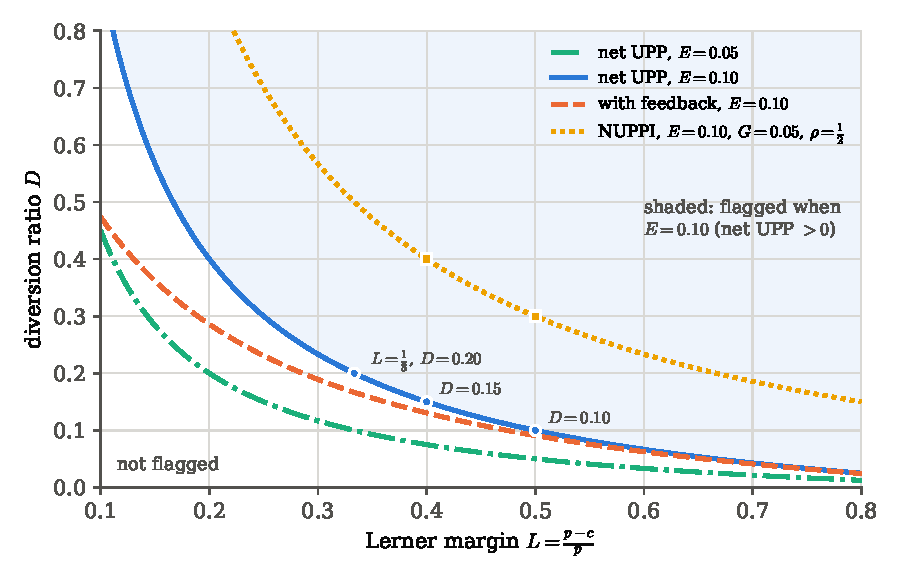
\includegraphics[width=0.86\textwidth]{figures/ch11/upp_thresholds.pdf}
\caption{UPP screening thresholds for a symmetric merger. Each curve gives the diversion ratio above which a test flags
the merger. The tests are net UPP with default efficiencies of 5 and 10 percent \eqref{eq:11-fs2}, the feedback test
\eqref{eq:11-fs4}, and the NUPPI test \eqref{eq:11-nuppi-sym} with $G = 0.05$ and $\rho = \frac{1}{2}$. The shaded
region is flagged by net UPP with $E = 0.10$. Circles mark the three cases in Farrell and Shapiro's fn.~43 and p.~17,
and squares mark their two NUPPI cases on p.~21.}
\label{fig:11-uppregion}
\end{figure}

\casehead{Extensions} The cannibalization logic extends in several directions
\citep[Sections 2.F and 7]{FarrellShapiro2010}. If firm A sells only product 1 while firm B sells products
$2, \dots, n$, the same derivation gives the tax
\begin{equation}\label{eq:11-upp-multi}
  t_1 = \sum_{j=2}^{n} D_{1j}\,(p_j - c_j) .
\end{equation}
When B's products have similar absolute margins, only the aggregate diversion from product 1 to B's group is needed.
If B sells a complement to product 1, say product 3, then $D_{13} < 0$. The merged firm then wants to lower $p_1$ to
spur sales of product 3, and the term $D_{13}(p_3 - c_3)$ offsets the pressure from substitutes. Follow-on revenues
enter through the margin. With spare parts, network effects, learning by doing or switching costs, a sale of product
2 today brings profits later, and the effective margin on product 2 exceeds $p_2 - c_2$. Accounting records sometimes
value these gains, and they usually make UPP for product 1 more likely.

Farrell and Shapiro derived \eqref{eq:11-upp} under static Bertrand pricing. If firms accommodate each other's price
changes before the merger, there is less competition for the merger to eliminate, and the compensating efficiency is
smaller. They still recommend the simple test, leaving non-Bertrand conduct to the rebuttal stage. Otherwise a merger
could permanently remove competition that the parties have only temporarily softened. Under Cournot competition, the
formula holds with a diversion ratio of one (their fn.~36). To see why, let A choose $q_1$ in a homogeneous-goods
market with inverse demand $P(Q)$. After the merger, A internalizes $\frac{d\pi_B}{dq_1} = q_2 P'(Q)$, because B's
quantity is fixed and only the price falls. The per-unit tax is $-q_2 P'(Q)$. B's Cournot condition
$P - c_2 + q_2 P'(Q) = 0$ gives $-q_2P'(Q) = P - c_2$, so $t_1 = 1 \cdot (P - c_2)$.

\casehead{Rebuttal} Farrell and Shapiro intend the test as a presumption that the merging parties can rebut
(their Section 4). The parties can dispute the inputs, for example by showing that marginal costs are closer to prices
or that efficiencies exceed the standard deduction. They can argue that pass-through is low, so that pressure moves
prices little. This argument is irrelevant to the pure sign test. When the test flags only one product, they can argue
that neither price will rise. They can also argue that the consumer gain from a price cut on the other product
outweighs the harm from the increase.
Finally, a full analysis can consider repositioning, entry and verified efficiencies.

\casehead{Interpretation} UPP reframes the loss of competition as an increase in the merged firm's opportunity cost.
That cost is directly comparable with marginal-cost savings. The test answers a narrow question: does the merger
change pricing incentives upward on balance at pre-merger prices? It does not predict magnitudes. In return it needs
only margins and diversion, both of which antitrust agencies often observe from documents and data, and it avoids
drawing market boundaries. Margins are hard to measure in cross-industry academic work, but firms track their own
costs closely, and agencies can obtain those records.

\casehead{Critiques} Without efficiencies, every merger of substitutes creates positive UPP. The policy content of the
test therefore lies in the standard deduction $E$, or in the threshold $G$ of the NUPPI variant below. These
parameters are not derived from evidence on merger efficiencies. Because the test is a sign test, it cannot rank
mergers by harm. Two mergers with equal UPP can have very different price effects when pass-through differs, a point
that motivates the first-order approach of \citet{JaffeWeyl2013}. The Bertrand assumption, the measurement of
marginal cost and the use of diversion at pre-merger prices are further sources of error. The test also ignores
repositioning and entry. \citet{MillerEtAl2017} compare UPP-based predictions with full merger simulations in
simulated industries.

\casehead{Contribution} Farrell and Shapiro made explicit the economic core of unilateral effects. A merger raises
the merged firm's effective marginal cost by the diversion-weighted margin of the partner product. They showed that the sign of the price effect is much easier to establish than its size. Their
framework, together with GUPPI, moved the analysis of unilateral effects away from market shares and toward diversion
and margins.

\subsection{From pricing pressure to price changes: pass-through}\label{sec:11-passthrough}

Under the conditions of \cref{prop:11-fs2}, the price effect of a merger equals the price response to a cost
increase on the merging products. That response is a \emph{pass-through rate}. It is the pass-through of a cost shock to some
products only, and it is an equilibrium rate, including rivals' responses. We first derive single-product pass-through
and then the multi-product approximation of \citet{JaffeWeyl2013}. \Cref{ch:theory} treats pass-through in general.

\begin{lemma}[Single-product pass-through]\label{lem:11-passthrough}
Let a firm face demand $q(p)$, holding rivals' prices fixed, with constant marginal cost $c$. Suppose the profit
maximizing price satisfies the first-order condition $q + (p - c)q' = 0$ and the second-order condition
$2q' + (p - c)q'' < 0$. Then
\begin{equation}\label{eq:11-passthrough}
  \rho = \frac{dp}{dc} = \frac{1}{2 + L\psi} , \qquad \psi = \frac{p\,q''(p)}{q'(p)} ,
\end{equation}
where $L = \frac{p - c}{p}$. Equivalently, with $\varepsilon(p) = -\frac{p\,q'(p)}{q(p)}$,
$\rho = \frac{\varepsilon}{\varepsilon - 1 + \frac{p}{\varepsilon}\frac{d\varepsilon}{dp}}$ \citep{BulowPfleiderer1983}.
\end{lemma}

\begin{proof}
Differentiate the first-order condition totally with respect to $p$ and $c$:
\begin{equation*}
  q'\,dp + q'\,(dp - dc) + (p - c)\,q''\,dp = 0 .
\end{equation*}
Collecting terms, $[2q' + (p-c)q'']\,dp = q'\,dc$, so $\rho = \frac{q'}{2q' + (p-c)q''}$. Dividing numerator and
denominator by $q'$, and writing $\frac{(p - c)q''}{q'} = \frac{p - c}{p}\cdot\frac{p\,q''}{q'} = L\psi$, gives
\eqref{eq:11-passthrough}. For the elasticity form, write the first-order condition as
$p\big[1 - \frac{1}{\varepsilon(p)}\big] = c$ and differentiate:
$\big[1 - \frac{1}{\varepsilon} + \frac{p}{\varepsilon^2}\frac{d\varepsilon}{dp}\big]dp = dc$. Solving for
$\frac{dp}{dc}$ and multiplying numerator and denominator by $\varepsilon$ gives the stated expression.
\end{proof}

Pass-through falls as demand becomes more elastic at higher prices. Three cases recur.

\begin{enumerate}[label=(\alph*)]
\item \emph{Linear demand.} Here $q'' = 0$, so $\psi = 0$ and $\rho = \frac{1}{2}$.
\item \emph{Constant elasticity.} With $q = k p^{-\varepsilon}$, $q' = -\varepsilon k p^{-\varepsilon - 1}$ and
      $q'' = \varepsilon(\varepsilon + 1)k p^{-\varepsilon - 2}$, so $\psi = -(\varepsilon + 1)$. The Lerner condition
      gives $L = \frac{1}{\varepsilon}$. Hence $\rho = \frac{1}{2 - \frac{\varepsilon + 1}{\varepsilon}} =
      \frac{\varepsilon}{\varepsilon - 1} = \frac{1}{1 - L} = \frac{p}{c} > 1$.
\item \emph{Logit, holding rivals' prices fixed.} The logit Lerner condition is $p - c = \frac{1}{\alpha(1 - s)}$.
      Differentiating, $dp - dc = \frac{1}{\alpha(1 - s)^2}\,ds$. Substituting $ds = -\alpha s(1 - s)\,dp$,
      \begin{equation*}
        dp - dc = -\frac{s}{1 - s}\,dp
        \quad\Longrightarrow\quad
        \frac{dp}{1 - s} = dc
        \quad\Longrightarrow\quad
        \rho = 1 - s .
      \end{equation*}
\end{enumerate}
Convex demand ($q'' > 0$, so $\psi < 0$) gives pass-through above one half, and concave demand gives less. Most
functional forms used in practice are convex.

Pass-through in oligopoly also depends on rivals' responses. In a Cournot market with linear inverse demand
$P = a - Q$ and $N$ active firms, firm $i$'s condition is $a - Q - q_i - c_i = 0$. Summing over firms gives
$Na - (N+1)Q = \sum_i c_i$, so $P = \frac{a + \sum_i c_i}{N + 1}$ and the pass-through of a firm-specific cost shock is
$\frac{1}{N+1}$ \citep{BergstromVarian1985}. With differentiated products the intuition that competitive industries
pass through little can fail. A firm facing very elastic residual demand prices close to cost before and after a cost
shock, so its pass-through is near one. Under constant elasticity it exceeds one \citep[Section 3.D]{FarrellShapiro2010}.

\casehead{The first-order approach} \citet{JaffeWeyl2013} turn \cref{prop:11-fs2} into an approximation. Divide each
first-order condition by $-\frac{\partial q_j}{\partial p_j}$ and write the pricing conditions in per-unit form,
\begin{equation}\label{eq:11-foa-f}
  f_j(p;\Omega) = p_j - c_j - \frac{q_j(p)}{-\frac{\partial q_j(p)}{\partial p_j}}
  - \sum_{k \ne j} \Omega_{jk}\, D_{jk}(p)\,(p_k - c_k) = 0 .
\end{equation}
For single-product firms before the merger the sum is empty. After the merger, the condition for product 1 gains the
term $D_{12}(p)(p_2 - c_2)$. Hence $f^{post}(p) = f^{pre}(p) - g(p)$, where $g(p)$ is the vector of generalized pricing
pressures. At the pre-merger prices $f^{pre}(p^0) = 0$, so $f^{post}(p^0) = -g(p^0)$, whose entries are $-\mathit{UPP}_j$
for the merging products and zero for others. A first-order expansion of $f^{post}(p^1) = 0$ around $p^0$ gives
\begin{equation*}
  0 = f^{post}(p^1) \approx f^{post}(p^0) + J^{post}\,(p^1 - p^0) , \qquad J^{post} = \frac{\partial f^{post}}{\partial p}(p^0) ,
\end{equation*}
and therefore
\begin{equation}\label{eq:11-foa}
  p^1 - p^0 \approx \big[J^{post}\big]^{-1} \mathit{UPP} \equiv \rho^{post}\, \mathit{UPP} .
\end{equation}
The matrix $\rho^{post}$ is a pass-through matrix. If each product's effective marginal cost rises by a per-unit amount
$\tau_j$, the conditions become $f^{post}(p) - \tau = 0$, and the implicit function theorem gives
$\frac{dp}{d\tau} = [J^{post}]^{-1}$. The merger price effect is approximately merger pass-through times UPP. Here $\tau$
shifts each normalized first-order condition directly. A rise in a physical marginal cost $c_k$ also changes the partner
term $D_{jk}(p_k - c_k)$. With $B_{jk} = \Omega_{jk}D_{jk}$ for $k \ne j$ and $B_{jj} = 0$,
\eqref{eq:11-foa-f} gives $f(p; c + \tau) = f(p; c) - (I - B)\tau$, so physical-cost pass-through is
$\frac{dp}{dc} = [J^{post}]^{-1}(I - B)$. The two coincide for single-product firms, where $B = 0$. The
pre-merger cost pass-through matrix $[J^{pre}]^{-1}$ can sometimes be estimated from past cost shocks. Jaffe and Weyl
propose using it in place of $\rho^{post}$ when demand curvature cannot be estimated directly. In the logit example of
\cref{sec:11-logitex}, the approximation \eqref{eq:11-foa} predicts a merging-firm price of 1.0648 with post-merger
pass-through and 1.0635 with pre-merger pass-through. The exact post-merger price is 1.0637.

\casehead{Curvature drives predictions} Because pass-through depends on second derivatives of demand, predicted merger
effects depend on curvature, which data rarely pin down. In practice curvature is set by the choice of functional
form. \citet{FroebTschantzWerden2005} simulated the proposed MCI and Sprint merger and found that constant-elasticity
demand predicted price effects over seven times larger than linear demand \citep[p.~19]{FarrellShapiro2010}. They also
noted that demand systems with higher pass-through of efficiencies predict larger price effects without efficiencies.
\Cref{prop:11-fs2} explains this pattern: both quantities are pass-through rates. \citet{CrookeEtAl1999} document the
same sensitivity across standard functional forms.

\Cref{fig:11-curvature} isolates the role of curvature. Two symmetric firms merge, and each demand system is calibrated
to the same price, marginal cost, own-price elasticity and diversion ratio at the pre-merger equilibrium. The
\emph{constant-expenditure logit} applies the logit formula, with log price in utility, to expenditure shares
(\cref{sec:11-bv}). Under linear, logit and constant-expenditure logit demand the merged firm's joint profit is
bounded. A grid search over both prices puts its global maximum at the symmetric solution of the first-order
conditions. The constant-expenditure logit, whose elasticities change little with price, predicts 2.4 to 3.3 times
the linear effect over the plotted range. Logit lies between linear and the constant-expenditure logit.

Constant-elasticity demand needs care. Hold $p_1 > c$ fixed and raise $p_2$. Then $q_1$ grows without bound, while
product 2 earns a nonnegative profit, so joint profit has no maximum for any $D > 0$. The figure therefore shows the
merged firm's optimum when it must charge one common price for both products. That price also solves the symmetric
first-order conditions that a merger simulation would solve. The implied price increase is 3.3 to 5.2 times the
linear effect. Without the restriction the symmetric solution is a strict local maximum of joint profit only for $D$
below about 0.25 and a saddle point above. Constant-elasticity demand is thus a local approximation, and its merger
predictions rely on that approximation far from observed prices.

The figure also plots the prediction obtained by freezing shares and slopes at their
pre-merger values, which we show in \cref{sec:11-simframework} equals the compensating cost reduction. Linear demand
predicts exactly half of it, because the symmetric linear pass-through of a cost shock to both products is one half.
\Cref{sec:11-bv} shows that the same issue separated the predictions of unit-demand and constant-expenditure
specifications in a merger of analgesics producers.

\begin{figure}[htbp]
\centering
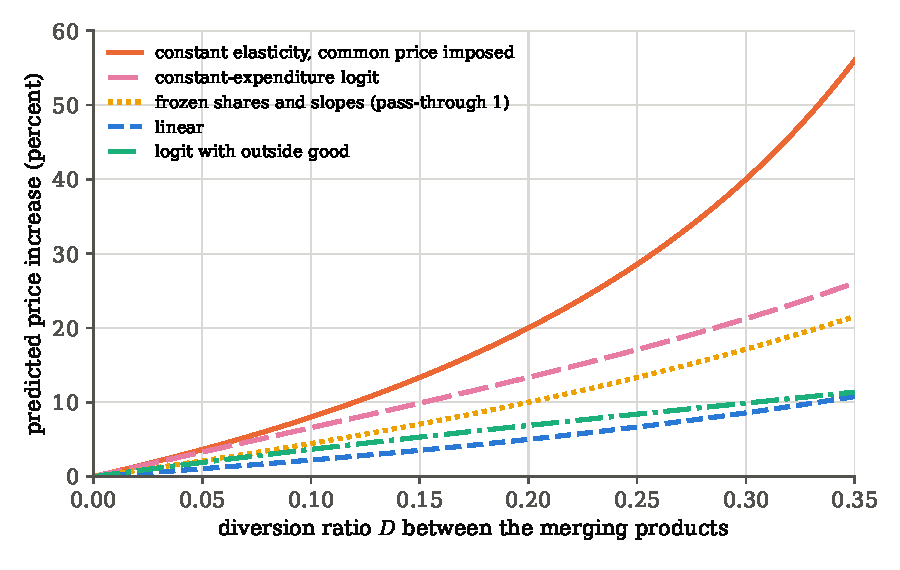
\includegraphics[width=0.86\textwidth]{figures/ch11/curvature_sim.pdf}
\caption{Predicted price increase from a merger of two symmetric single-product firms under four demand systems with
identical first derivatives at the pre-merger point. Calibration: $p = 1$, $c = 0.6$ ($L = 0.4$), own-price elasticity
$2.5$, diversion $D$ between the merging products on the horizontal axis, no efficiencies. Linear:
$q_j = a - b p_j + d p_k$ with $b = 2.5$ and $d = 2.5D$. Logit: one outside good, inside shares $\frac{D}{1+D}$.
Constant-expenditure logit: one outside good, value shares $w_j$ proportional to $p_j^{-\alpha}$ with
$\alpha = 1.5 + 2.5D$, and $q_j = \frac{B w_j}{p_j}$. Constant elasticity: $q_j = k p_j^{-2.5} p_k^{2.5 D}$, with the
merged firm restricted to one common price because its unrestricted joint profit is unbounded. The dotted line
freezes shares and slopes at pre-merger values, which gives $\frac{D L}{1 - D}$. Source: our calculations.}
\label{fig:11-curvature}
\end{figure}

\casehead{A significance threshold: NUPPI} Merger practice often asks first whether a merger without efficiencies would
cause a ``significant'' price increase, say a fraction $G$ of the price \citep[Section 3.C]{FarrellShapiro2010}. Let
$\rho_1$ be the equilibrium pass-through of a cost shock to product 1 alone. Internalizing the first-round tax raises
$p_1$ significantly if $\rho_1 t_1 > G p_1$. Dividing by $\rho_1 p_1$ gives inequality (5),
\begin{equation}\label{eq:11-fs5}
  D_{12}\,\frac{p_2 - c_2}{p_2}\,\frac{p_2}{p_1} > \frac{G}{\rho_1} ,
\end{equation}
which is $\mathit{GUPPI}_1 > \frac{G}{\rho_1}$. Adding the efficiency credit, $\rho_1[D_{12}(p_2 - c_2) - E c_1] > G p_1$,
which after dividing by $\rho_1 p_1$ becomes inequality (6),
\begin{equation}\label{eq:11-fs6}
  D_{12} L_2 \frac{p_2}{p_1} - E_1 (1 - L_1) > \frac{G}{\rho_1} .
\end{equation}
Farrell and Shapiro call the left side the \emph{net upward pricing pressure index} (NUPPI). In the symmetric case,
with $\rho$ the pass-through of a cost increase on both products,
\begin{equation}\label{eq:11-nuppi-sym}
  D L - E(1 - L) > \frac{G}{\rho} .
\end{equation}
Since $\rho$ is hard to estimate, a screen needs a default. They suggest $\rho = \frac{1}{2}$, the single-firm rate with
linear demand, which rivals' accommodation would raise (their fn.~59). With $G = 0.05$ and $\rho = \frac{1}{2}$, the
merger is presumed harmful when NUPPI is at least 10 percent. With $E = 0.10$, NUPPI equals $(D + 0.1)L - 0.1$, so the
condition is $(D + 0.1)L > 0.2$. A margin of 0.4 requires $D > 0.40$, and a margin of 0.5 requires $D > 0.30$
(p.~21). The NUPPI test is far more permissive than \eqref{eq:11-fs1}, especially with low assumed pass-through. It also
describes the roundabout way efficiencies enter merger review. Agencies first ask whether the merger without
efficiencies raises price significantly, which is \eqref{eq:11-fs6} with $E_1 = 0$ and needs a view on $\rho_1$. They
then ask whether efficiencies offset the gross pressure, which is \eqref{eq:11-fs6} with $G = 0$.

\casehead{UPP, simulation and market definition} Farrell and Shapiro compare their test with the two alternatives
(their Sections 5 and 6). Merger simulation must estimate the pass-through of the asymmetric cost shock in
\cref{prop:11-fs2}, explicitly or implicitly. Its predictions therefore depend heavily on the assumed demand system,
which invites a battle of experts. Simulation also tries to explain price levels, so it risks misspecification from
omitted features of conduct. UPP looks at the change in marginal incentives, which nets out features present before
and after the merger. Market definition is less different from simulation than it appears. The hypothetical monopolist
test simulates a merger of all products in a candidate market, and so it also hinges on pass-through. Only the sign
test avoids pass-through. Farrell and Shapiro suggest that a court could keep a broad market definition for context
while the government establishes its presumption through UPP within that market.

\section{Merger simulation}\label{sec:11-simulation}

Merger simulation predicts the post-merger equilibrium from an estimated model of demand and an assumed model of
conduct. \citet{BakerBresnahan1985}, \citet{HausmanLeonardZona1994} and \citet{WerdenFroeb1994} developed the approach
with residual demand, multi-level demand and logit demand. \citet{Nevo2000b} combined it with random coefficients
demand and computed full equilibria and welfare. This section sets out the general framework, works a logit example
in detail and then studies Nevo's application to ready-to-eat cereal.

\subsection{The framework}\label{sec:11-simframework}

Consider one market with $J$ products and market size $M$. Firm $f$ owns the products $\mathcal{J}_f$ and earns
\begin{equation*}
  \Pi_f = \sum_{j \in \mathcal{J}_f} (p_j - mc_j)\, M s_j(p) - C_f .
\end{equation*}
Under static multi-product Bertrand pricing (\cref{ch:diffprod,ch:blp}), the first-order condition for $j \in
\mathcal{J}_f$ is
\begin{equation}\label{eq:11-foc-multi}
  s_j(p) + \sum_{k \in \mathcal{J}_f} (p_k - mc_k)\frac{\partial s_k(p)}{\partial p_j} = 0 .
\end{equation}
Let $\Omega$ be the ownership matrix, with $\Omega_{jk} = 1$ when $j$ and $k$ have the same owner. Since the $(j,k)$
element of $\Delta^\top$ is $\frac{\partial s_k}{\partial p_j}$, stacking \eqref{eq:11-foc-multi} gives
\begin{equation}\label{eq:11-foc-matrix}
  s(p) + \big(\Omega \odot \Delta(p)^\top\big)(p - mc) = 0
  \quad\Longleftrightarrow\quad
  p = mc - \big(\Omega \odot \Delta(p)^\top\big)^{-1} s(p) .
\end{equation}
Because ownership is symmetric, $\Omega \odot \Delta^\top = (\Omega \odot \Delta)^\top$. \citet{Nevo2000b} writes the
same system with a matrix whose $(j,k)$ element is $-\frac{\partial s_j}{\partial p_k}$ for jointly owned products. That
is the transpose of ours. The difference is immaterial when the Jacobian is symmetric, as in logit, nested logit and
random coefficients logit with utility linear in price. It matters when price enters utility as $-\alpha \ln p_j$,
because then $\frac{\partial s_k}{\partial p_j} = \frac{\alpha s_j s_k}{p_j}$ is not symmetric.

\begin{assumption}[Merger simulation]\label{ass:11-sim}
(i) Demand is stable across the merger: the same function $s(p)$ applies before and after. (ii) Before the merger,
prices form a Bertrand-Nash equilibrium under $\Omega^{pre}$. (iii) After the merger, prices form a Bertrand-Nash
equilibrium under $\Omega^{post}$, which sets $\Omega_{jk} = 1$ for every pair of the merging firms' products.
(iv) Marginal costs are constant and unchanged by the merger unless efficiencies are imposed. (v) The set of products
and all non-price choices are fixed.
\end{assumption}

The algorithm has five steps.
\begin{enumerate}[label=(\arabic*)]
  \item Estimate demand on pre-merger data. This delivers $s(\cdot)$ and $\Delta(\cdot)$.
  \item Recover marginal costs from the pre-merger conditions,
        \begin{equation}\label{eq:11-mc-recover}
          \widehat{mc} = p^{pre} + \big(\Omega^{pre} \odot \Delta(p^{pre})^\top\big)^{-1} s(p^{pre}) .
        \end{equation}
  \item Replace $\Omega^{pre}$ by $\Omega^{post}$. Optionally lower the merging firms' costs to represent efficiencies.
  \item Solve \eqref{eq:11-foc-matrix} for the post-merger prices $p^*$ under $\Omega^{post}$ and the new costs.
  \item Compute the changes in prices, consumer surplus, profits and total welfare.
\end{enumerate}
Step 2 needs no cost data, but it relies on the pre-merger conduct assumption. \Cref{ch:blp} shows how cost shifters
can be added to estimate a supply side jointly with demand. \citet[eq.~(9)]{Nevo2000b} notes that
conduct parameters could multiply the entries of $\Omega$ and be estimated, but that this is hard in practice.

\casehead{The first iteration} Before Nevo's work, practitioners often reported an approximation instead of the
equilibrium \citep{HausmanLeonardZona1994,Werden1997}. It replaces the post-merger shares and derivatives by their
pre-merger values:
\begin{equation}\label{eq:11-approx}
  p^{approx} = \widehat{mc} - \big(\Omega^{post} \odot \Delta(p^{pre})^\top\big)^{-1} s(p^{pre})
\end{equation}
\citep[eq.~(11)]{Nevo2000b}. It is the first step of the fixed-point iteration on \eqref{eq:11-foc-matrix} started at
$p^{pre}$, so it captures the merged firm's direct incentive to raise price. The next result relates it to UPP.

\begin{proposition}[First iteration and compensating cost reductions]\label{prop:11-approx}
Let single-product firms 1 and 2 merge. The approximation \eqref{eq:11-approx} leaves every non-merging price unchanged.
For the merging products, $p_1^{approx} - p_1^{pre}$ and $p_2^{approx} - p_2^{pre}$ equal the compensating marginal
cost reductions $\Delta c_1$ and $\Delta c_2$ of \cref{prop:11-cmcr}.
\end{proposition}

\begin{proof}
Write $m = p^{pre} - \widehat{mc}$ for the pre-merger margins and $m' = p^{approx} - \widehat{mc}$. By step 2 and
\eqref{eq:11-approx}, both satisfy linear systems with the same right side:
\begin{equation*}
  \big(\Omega^{post} \odot \Delta^\top\big) m' = -s = \big(\Omega^{pre} \odot \Delta^\top\big) m ,
\end{equation*}
with $s$ and $\Delta$ at $p^{pre}$. Both matrices are block diagonal by owner. The blocks of non-merging firms coincide,
so their margins are unchanged. The merging block has rows
\begin{equation*}
  \frac{\partial s_1}{\partial p_1} m_1' + \frac{\partial s_2}{\partial p_1} m_2' = \frac{\partial s_1}{\partial p_1} m_1 , \qquad
  \frac{\partial s_1}{\partial p_2} m_1' + \frac{\partial s_2}{\partial p_2} m_2' = \frac{\partial s_2}{\partial p_2} m_2 .
\end{equation*}
Dividing the first row by $-\frac{\partial s_1}{\partial p_1}$ gives $-m_1' + D_{12} m_2' = -m_1$, so
$m_1' - m_1 = D_{12}\big(m_2 + (m_2' - m_2)\big)$. The second row gives $m_2' - m_2 = D_{21}\big(m_1 + (m_1' - m_1)\big)$.
These are the equations for $\Delta c_1$ and $\Delta c_2$ in the proof of \cref{prop:11-cmcr}, with margins
$p_j - c_j = m_j$. Their unique solution is \eqref{eq:11-cmcr}.
\end{proof}

The first iteration is therefore UPP with feedback between the merging products and with a pass-through of exactly
one. The compensating cost reduction is the cost cut that would offset the merger. The first iteration is the price
increase that the merger would cause if every unit of pricing pressure passed into price. The approximation overstates
the equilibrium effect when pass-through is below one, as with logit demand and small shares. It understates the effect
when pass-through exceeds one, as with the constant-expenditure logit of \cref{fig:11-curvature}.

\casehead{Computation} Solving \eqref{eq:11-foc-matrix} means solving $J$ nonlinear equations. The usual choice is a
Newton or quasi-Newton method applied to the first-order conditions, started from the pre-merger prices.
\citet[fn.~13]{Nevo2000b} used a standard nonlinear equation solver, and each city took several seconds on a 1997
personal computer. The naive iteration $p \leftarrow mc - (\Omega \odot \Delta(p)^\top)^{-1}s(p)$ need not converge.
\citet{MorrowSkerlos2011} propose a better-behaved fixed point for logit-type demand in which price enters utility as
$-\alpha_i p_j$. Decompose the Jacobian as $\Delta = \Lambda - \Gamma$, where the diagonal matrix $\Lambda$ has entries
$\Lambda_{jj} = -\int \alpha_i s_{ij}\,dP(i)$ and $\Gamma_{jk} = -\int \alpha_i s_{ij}s_{ik}\,dP(i)$. These two matrices
follow the notation of Morrow and Skerlos and are unrelated to the scalars $\Lambda$ of \cref{sec:11-fs} and $\Gamma$
of \cref{sec:11-dd}. Substituting into \eqref{eq:11-foc-matrix} and using $\Omega \odot \Lambda = \Lambda$,
\begin{equation}\label{eq:11-zeta}
  p = mc + \zeta(p) , \qquad \zeta(p) = \Lambda(p)^{-1}\big[\big(\Omega \odot \Gamma(p)^\top\big)(p - mc) - s(p)\big] .
\end{equation}
They report that iterating on this map is fast and reliable in large problems, and \texttt{pyblp} uses it
(\cref{ch:blp}). Existence and uniqueness of the post-merger equilibrium are not automatic. The log-concavity
conditions of \citet{CaplinNalebuff1991} give existence for broad classes of discrete choice demand when each firm
sells one product (\cref{thm:04-cn-existence}). Their uniqueness results cover only restricted cases, such as the
logit and duopoly (\cref{sec:04-uniqueness}). A merger creates a multiproduct firm, which their theorems do not cover.
With logit demand, uniqueness holds for every ownership structure (\cref{thm:04-logit-unique}). Random coefficients
demand with multiproduct firms has no such theorem. In practice one checks that the solver reaches the same prices
from several starting points.

\casehead{Calibration} The simulated pre-merger prices must equal observed prices, so that the simulation compares the
merger with the status quo. In a logit model one can add a residual to predicted shares. \citet[p.~31]{Nevo2000b}
points out that with heterogeneous consumers this can make individual purchase probabilities negative. He adds the
estimated residual $\xi$ to utility instead, so that the model reproduces observed shares exactly.

\casehead{Welfare} With utility linear in price and type I extreme value errors, the expected consumer surplus of
consumer $i$, up to a constant, is
\begin{equation}\label{eq:11-cs}
  \mathit{CS}_i = \frac{1}{\alpha_i}\ln\Big(1 + \sum_{j=1}^{J} e^{V_{ij}}\Big) .
\end{equation}
Here $V_{ij}$ is the deterministic part of utility from product $j$. The outside good has $V_{i0} = 0$
\citep{SmallRosen1981,Trajtenberg1989}. The log-sum is the expected maximum utility. Dividing by $\alpha_i$, the
marginal utility of income, converts it into money (\cref{ch:logit}). The change in consumer surplus is
\begin{equation}\label{eq:11-dcs}
  \Delta \mathit{CS} = M\,\frac{1}{n_s}\sum_{i=1}^{n_s} \frac{1}{\alpha_i}
  \Big[\ln\Big(1 + \sum_j e^{V_{ij}^{post}}\Big) - \ln\Big(1 + \sum_j e^{V_{ij}^{pre}}\Big)\Big] ,
\end{equation}
averaging over $n_s$ simulated consumers. With plain logit, $\alpha_i = \alpha$ and the average has one term. The change
in producer surplus is $\sum_j (p_j^{post} - mc_j^{post}) M s_j^{post} - \sum_j (p_j^{pre} - mc_j^{pre}) M s_j^{pre}$,
since fixed costs are unchanged. Total welfare changes by the sum.

\casehead{Partial internalization} The framework accommodates objectives that place weight on other firms' profits.
Suppose firm $f$ maximizes $\Pi_f + \sum_{g \ne f} \kappa_{fg}\Pi_g$. The first-order condition keeps the form
\eqref{eq:11-foc-matrix} with $\Omega_{jk}(\kappa) = \kappa_{fg}$ for $j \in \mathcal{J}_f$ and $k \in \mathcal{J}_g$.
With partial ownership, \citet{OBrienSalop2000} derive the weights from financial interests and control rights.
\citet{MillerWeinberg2017} use a common weight $\kappa$ to measure coordination between two firms after a joint venture
(\cref{sec:11-millercoors}). When $\kappa_{fg} \ne \kappa_{gf}$, $\Omega$ is not symmetric, and the form
$\Omega \odot \Delta^\top$ in \eqref{eq:11-foc-matrix} must be used.

\casehead{Caveats} A simulation is only as good as the demand model. Functional form fixes curvature and hence
pass-through (\cref{sec:11-passthrough}). Simulation also relies on assumptions about post-merger conduct: joint profit
maximization, unchanged behavior of rivals, a stable demand system and predictable efficiencies. Nevo stresses that
$\Omega^{pre}$ and $\Omega^{post}$ use the same demand estimates. This is inconsistent with firms changing other choices
that affect demand. If advertising changes after the merger and affects $\frac{\partial s}{\partial p}$, the predicted
prices are wrong. Product repositioning, entry and new products are absent from the static model
\citep[pp.~23--25]{Nevo2000b}. Finally, the exercise is data-intensive and time-consuming, which matters under the
statutory deadlines of merger review.

\subsection{A worked example with logit demand}\label{sec:11-logitex}

The following example traces every concept of this section and \cref{sec:11-upp} through one calibrated market. The
calibration is the one \citet[p.~1780]{MillerWeinberg2017} use to illustrate their internalization parameter. All
numbers are our computations.

\begin{example}[Logit merger simulation]\label{ex:11-logit}
Three symmetric single-product firms sell at $p = 1$ with marginal cost $c = 0.7$. Each has share $s = 0.2$, and the
outside good has $s_0 = 0.4$. Market size is one. Demand is logit, and pre-merger prices are a Bertrand-Nash
equilibrium. Firms 1 and 2 merge.

\emph{Calibration.} The logit Lerner condition $p - c = \frac{1}{\alpha(1 - s)}$ gives
$\alpha = \frac{1}{0.3 \times 0.8} = 4.1667$. Mean utilities satisfy $e^{\delta_j} = \frac{s_j}{s_0} = 0.5$.

\emph{Screening statistics.} Diversion is $D_{12} = \frac{0.2}{1 - 0.2} = 0.25$, and diversion to the outside good is
$\frac{0.4}{0.8} = 0.5$. Upward pricing pressure is $\mathit{UPP}_1 = 0.25 \times 0.3 = 0.075$, so
$\mathit{GUPPI}_1 = 7.5$ percent. With $L = 0.3$ and $E = 0.10$, the simple test requires
$D > \frac{0.1 \times 0.7}{0.3} = 0.233$, which holds narrowly. Net UPP is $0.075 - 0.07 = 0.005$. The feedback test
compares $\frac{D}{1 - D} = 0.333$ with $0.233$ and flags the merger clearly. By \eqref{eq:11-cmcr}, the compensating
cost reduction is
\begin{equation*}
  \Delta c = \frac{0.25 \times 0.3 + 0.0625 \times 0.3}{1 - 0.0625} = 0.100 ,
\end{equation*}
which is 14.3 percent of marginal cost. A 10 percent standard deduction falls short.

\emph{Approximations.} Holding the rival's price fixed, single-product logit pass-through is $1 - s = 0.8$, so
$\rho\,\mathit{UPP} = 0.06$. The first iteration \eqref{eq:11-approx} gives $p_1 = p_2 = 1.100$ and $p_3 = 1$, the
compensating reduction of \cref{prop:11-approx}. The first-order approach \eqref{eq:11-foa} gives 1.0648 with
post-merger pass-through and 1.0635 with pre-merger pass-through. Farrell and Shapiro's iterative tax procedure
converges within three rounds. The first round imposes taxes of 0.075 and yields prices of 1.0641. The second round
lowers the taxes to 0.0745 and the prices slightly, to 1.0637. The third round changes neither at four decimals. The
limiting tax of
\cref{prop:11-fs2} is $t^* = 0.2049 \times 0.3637 = 0.0745$. It is slightly below the first-round tax: the margin rises,
but diversion falls from 0.25 to 0.2049 as the merging products' shares fall.

\emph{Full simulation.} The post-merger equilibrium prices are $(1.0637, 1.0637, 1.0062)$. The merging firms raise
prices by 6.4 percent and the rival by 0.6 percent. The merged firm's markup of 0.3637 equals the multi-product logit
common markup $\frac{1}{\alpha(1 - S_f)}$ with combined share $S_f = 0.3402$ (\cref{ch:diffprod,app:problems}). Consumer
surplus falls by 0.0249, against pre-merger revenue of 0.6. The merged firm's profit rises by 0.0037, and the rival's by
0.0062. Total welfare falls by 0.0149.

\emph{Efficiencies.} If the merger lowers the merging firms' cost to $0.7 - 0.1 = 0.6$, the post-merger equilibrium is
the pre-merger price vector. Consumers are unaffected, and total welfare rises by the cost saving of 0.04.

\emph{Partial internalization.} Suppose the merged firm and firm 3 each place weight $\kappa = 0.5$ on the other's
profit. Then prices rise to $(1.1040, 1.1040, 1.0731)$, and consumer surplus falls by 0.0515, about twice the loss
under unilateral effects alone. With the merging firms' cost cut to 0.5, prices are $(0.9834, 0.9834, 1.1028)$. The
efficiency lowers the merging firms' prices but raises firm 3's. The merging products' margins grow, and firm 3
internalizes half of them. Consumer surplus is unchanged only if the merging firms' cost falls to 0.4532, a 35.3
percent reduction, against 14.3 percent without coordination.
\end{example}

\begin{table}[htbp]
\centering
\caption{Logit merger example: prices, outside share and welfare changes}
\label{tab:11-logitex}
\small
\begin{tabular}{@{}lccccccc@{}}
\toprule
Scenario & $p_1 = p_2$ & $p_3$ & $s_0$ & $\Delta\mathit{CS}$ & $\Delta\pi_{1+2}$ & $\Delta\pi_3$ & $\Delta W$ \\
\midrule
Pre-merger                                   & 1.0000 & 1.0000 & 0.4000 & 0       & 0       & 0       & 0       \\
First iteration \eqref{eq:11-approx}         & 1.1000 & 1.0000 &        &         &         &         &         \\
First-order approach \eqref{eq:11-foa}       & 1.0648 & 1.0065 &        &         &         &         &         \\
Merger, $\kappa = 0$                         & 1.0637 & 1.0062 & 0.4436 & $-0.0249$ & 0.0037 & 0.0062 & $-0.0149$ \\
Merger, $\kappa = 0$, $c_{1,2} = 0.6$         & 1.0000 & 1.0000 & 0.4000 & 0.0000  & 0.0400  & 0.0000  & 0.0400  \\
Merger, $\kappa = 0.5$                       & 1.1040 & 1.0731 & 0.4958 & $-0.0515$ & 0.0099 & 0.0082 & $-0.0335$ \\
Merger, $\kappa = 0.5$, $c_{1,2} = 0.68$      & 1.0907 & 1.0755 & 0.4877 & $-0.0476$ & 0.0173 & 0.0069 & $-0.0235$ \\
Merger, $\kappa = 0.5$, $c_{1,2} = 0.5$       & 0.9834 & 1.1028 & 0.4171 & $-0.0101$ & 0.0961 & $-0.0053$ & 0.0807 \\
Merger, $\kappa = 1$                         & 1.1405 & 1.1405 & 0.5449 & $-0.0742$ & 0.0137 & 0.0068 & $-0.0537$ \\
\bottomrule
\end{tabular}

\smallskip
\begin{minipage}{0.95\linewidth}
\footnotesize
Notes: Three symmetric firms with $p = 1$, $c = 0.7$, $s = 0.2$, $s_0 = 0.4$ and $\alpha = 4.1667$ before the merger.
Firms 1 and 2 merge. $\kappa$ is the weight that the merged firm and firm 3 place on each other's profit. $c_{1,2}$ is
the merging firms' post-merger marginal cost (0.7 unless stated). Welfare changes are per unit of market size and in
units of price, with consumer surplus from \eqref{eq:11-dcs}. The first-order approach row uses post-merger
pass-through. Source: our calculations.
\end{minipage}
\end{table}

\begin{figure}[htbp]
\centering
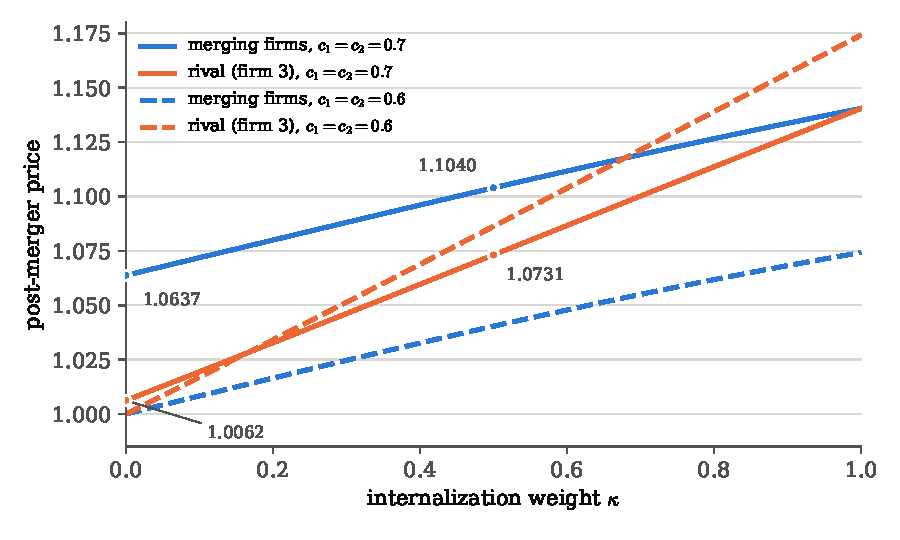
\includegraphics[width=0.86\textwidth]{figures/ch11/logit_kappa.pdf}
\caption{Post-merger prices in the logit example as a function of the internalization weight $\kappa$ between the
merged firm and firm 3. Solid lines keep the merging firms' marginal cost at 0.7, and dashed lines lower it to 0.6, the
compensating cost reduction. Dots mark $\kappa = 0$ and $\kappa = 0.5$. Source: our calculations.}
\label{fig:11-kappa}
\end{figure}

\Cref{fig:11-kappa} shows how $\kappa$ separates unilateral from coordinated effects. At $\kappa = 0$ the rival's price
barely moves, since its response comes only through strategic complementarity. As $\kappa$ rises, the rival's price
rises nearly linearly, and at $\kappa = 1$ the industry behaves as a monopoly. With the compensating cost reduction
(dashed lines), merging prices stay at one when $\kappa = 0$, but coordination still raises all prices. Efficiencies
can offset unilateral effects, but they do not offset coordinated effects. The rival's price is the observable that
distinguishes the two. \citet{MillerWeinberg2017} build their identification argument for $\kappa$ on this contrast
(\cref{sec:11-millercoors}).

\begin{remark}[The third case in Miller and Weinberg's illustration]\label{rem:11-mw-typo}
\citet[p.~1780]{MillerWeinberg2017} report post-merger prices of about 1.06, 1.06 and 1.01 at $\kappa = 0$ and about
1.10, 1.10 and 1.07 at $\kappa = 0.5$, which match our calculations.
For $\kappa = 0.5$ with the merging firms' marginal cost lowered to 0.50, the text reports prices of 1.09, 1.09 and 1.08.
We obtain $(0.9834, 0.9834, 1.1028)$ for that case. The reported values correspond to a merging-firm cost of about
0.68. We obtain a merging price of 1.09 at a cost of 0.679, with the rival at 1.0756. \Cref{sec:11-mc-theory}
inverts both reported prices jointly for $\kappa$ and the merging firms' cost.
\end{remark}

\subsection{Nevo (2000): mergers in ready-to-eat cereal}\label{sec:11-nevo}

\casehead{The question} \citet{Nevo2000b} asks whether a flexible demand model, estimated with standard scanner data,
can discipline merger analysis in a concentrated industry with many differentiated products. He also asks how much the
answer depends on two choices: the demand model and the decision to compute the full post-merger equilibrium instead of
an approximation. Nevo frames merger simulation as the analogue of market definition. The ``front end'' estimates
demand, and the ``back end'' simulates the merger. He argues that the debate should focus on the front end, because
the demand estimates largely determine the outcome. The working paper (November 1997) was published in the RAND
Journal of Economics in 2000. Our equation and table numbers follow the working paper.

\casehead{The critique of traditional analysis} Nevo describes the screen of the 1982 and 1984 Guidelines (printed
pp.~5--6). A merger was not challenged if the post-merger HHI was below 1,000. Between 1,000 and 1,800, increases below 100 points
were usually not challenged. Above 1,800, an increase of 50 points was the threshold for a challenge. He argues that
concentration indices measure competitive effects well only if products are equally spaced in characteristics. Under
logit demand, substitution depends only on shares, and share-based policy is then sensible \citep{Willig1991}. For
cereal, logit is inadequate. Consumer heterogeneity also makes it easy to argue that hot cereal or bagels belong in
the market, which yields broad markets and small shares. The 1992 Guidelines introduced unilateral effects, and
\citet{Shapiro1996} described their implementation through diversion ratios and margins. Practice then moved to
computing price increases from estimated elasticities, usually with an approximation.

\casehead{Demand options} With $J$ products, an unrestricted demand system has on the order of $J^2$ price
parameters. With 200 cereal brands and constant elasticities, that is 40,000 elasticities. Nevo discusses three
solutions (his Section 3.1).
\begin{enumerate}[label=(\alph*)]
  \item \emph{Symmetric representative-consumer models.} The CES utility of \citet{DixitStiglitz1977} imposes equal
        cross-price elasticities. The representative-consumer form of logit has utility
        $\sum_i a_i q_i - \sum_i q_i \ln q_i$ \citep{AndersonDePalmaThisse1992}. Its entropy term treats all products
        symmetrically, so substitution depends only on shares.
  \item \emph{Multi-stage budgeting} \citep{HausmanLeonardZona1994}. The bottom level is an AIDS model for brand $j$ in
        segment $g$, city $c$ and quarter $t$ (\cref{ch:aids}),
        \begin{equation}\label{eq:11-nevo-aids}
          s_{jct} = \alpha_{jc} + \beta_j \ln\Big(\frac{y_{gct}}{P_{gct}}\Big) + \sum_{k=1}^{J} \gamma_{jk}\ln p_{kct} + \varepsilon_{jct} .
        \end{equation}
        Here $s_{jct}$ is the dollar share of segment expenditure $y_{gct}$ (his eq.~(1)). The price index is the Stone
        index $\ln P_{gct} = \sum_{k \in g} s_{kct}\ln p_{kct}$ (eq.~(2)) or the exact AIDS index (eq.~(3)). A middle
        level allocates expenditure across segments, for example with the log-log form
        $\ln q_{gct} = \beta_g \ln y_{Rct} + \sum_{k} \gamma_k \ln \pi_{kct} + \alpha_{gc} + \varepsilon_{gct}$. A top
        level gives total cereal demand. Nevo notes that the middle levels used in practice do not satisfy the
        conditions for exact two-stage budgeting.
  \item \emph{Discrete choice} \citep{Berry1994,BerryLevinsohnPakes1995}. Products are projected onto a space of
        characteristics, so the number of parameters grows with the number of characteristics.
\end{enumerate}
He rules out the symmetric models for merger work unless time is binding. Multi-level models need an a priori
segmentation into small groups and assume that every consumer buys every variety. They are closer to classical demand
theory and faster to compute. Discrete choice models need product characteristics and distributional assumptions, and
they are computationally heavier.

\casehead{The industry} Ready-to-eat cereal has high concentration, high price-cost margins, high advertising to
sales ratios and frequent product introductions. Concentration is high at the firm level and lower at the brand level.
The leading brands have about 5 percent of the market and the smaller brands in the sample about 1 percent.
\Cref{tab:11-nevo-shares} reports firm shares. Kellogg's volume share fell from 41.4 percent in the first quarter of
1988 to 33.7 percent in the last quarter of 1992, while General Mills rose from 22.0 to 26.8 percent. The three-firm
concentration ratio stayed above 70 percent throughout. Private labels grew from 3.3 to 7.6 percent of volume.

\begin{table}[htbp]
\centering
\caption{Firm shares in ready-to-eat cereal, 1988--1992, in percent (Nevo 1997 working paper, Tables 1A and 1B)}
\label{tab:11-nevo-shares}
\small
\begin{tabular}{@{}lcccccc@{}}
\toprule
 & \multicolumn{3}{c}{Volume shares} & \multicolumn{3}{c}{Sales shares} \\
\cmidrule(lr){2-4}\cmidrule(lr){5-7}
 & 88Q1 & 90Q4 & 92Q4 & 88Q1 & 90Q4 & 92Q4 \\
\midrule
Kellogg        & 41.39 & 37.86 & 33.70 & 41.23 & 37.26 & 32.57 \\
General Mills  & 22.04 & 23.82 & 26.83 & 24.73 & 27.70 & 31.39 \\
Post           & 11.80 & 10.96 & 11.31 & 11.15 & 10.56 & 10.97 \\
Quaker Oats    &  9.93 &  7.66 &  7.40 &  9.46 &  7.30 &  6.94 \\
Ralston        &  4.86 &  6.60 &  5.18 &  5.12 &  7.03 &  5.45 \\
Nabisco        &  5.32 &  3.75 &  3.11 &  5.00 &  3.58 &  3.33 \\
\midrule
C3             & 75.23 & 72.64 & 71.84 & 77.11 & 75.52 & 74.93 \\
C6             & 95.34 & 90.65 & 87.53 & 96.69 & 93.43 & 90.65 \\
Private label  &  3.33 &  6.29 &  7.60 &  2.12 &  3.74 &  4.55 \\
\bottomrule
\end{tabular}

\smallskip
\begin{minipage}{0.86\linewidth}
\footnotesize
Notes: C3 and C6 are the combined shares of the three and six largest firms. The paper also reports 88Q4, 89Q4 and
91Q4. Source: \citet{Nevo2000b}, working paper Tables 1A and 1B, from IRI Infoscan data.
\end{minipage}
\end{table}

\casehead{Data} Shares and prices come from the IRI Infoscan database, collected by scanners in a national random sample
of supermarkets. The sample represents supermarkets with annual sales above \$2 million, which account for 82 percent of
US grocery sales. Data are aggregated to the brand, city and quarter. The sample has 24 brands, listed by segment in his
Table 2: all-family or basic, taste-enhanced wholesome, simple health nutrition, and kids. The estimation sample
covers 45 cities and 20 quarters from 1988 to 1992, so it has $24 \times 45 \times 20 = 21{,}600$ observations in 900
city-quarter markets. Quantity
is converted into servings. Market size is one serving per capita per day, and the outside share is the remainder. Price
is dollar sales divided by servings, deflated by a regional urban CPI. It is the average transaction price at the
register, before any coupons redeemed after purchase.

Advertising comes from the Leading National Advertisers database, summed over ten media. Nevo collected
characteristics from cereal boxes: calories from fat, sugar, fiber, segment dummies and a ``mushy'' dummy for cereals
that turn soggy in milk. Demographics are drawn from the March Current Population Survey (CPS): income per person
(household income divided by household size), age and a child dummy. Instruments use supermarket-sector wages by city
from CPS earnings files, city density, and regional price indices from the Bureau of Labor Statistics.

\casehead{The model} The indirect utility of consumer $i$ from brand $j$ in market $t$ is (his eq.~(4), in our sign
convention)
\begin{equation}\label{eq:11-nevo-u}
  u_{ijt} = x_{jt}\beta_i - \alpha_i p_{jt} + \xi_j + \Delta\xi_{jt} + \epsilon_{ijt} .
\end{equation}
Here $\xi_j$ is the national mean of unobserved quality and $\Delta\xi_{jt}$ the market-specific deviation. Tastes
depend on demographics $D_i$ and unobserved draws $\nu_i$ (eq.~(5)),
\begin{equation}\label{eq:11-nevo-rc}
  \begin{pmatrix} \alpha_i \\ \beta_i \end{pmatrix}
  = \begin{pmatrix} \alpha \\ \beta \end{pmatrix} + \Pi D_i + \Sigma \nu_i , \qquad \nu_i \sim N(0, I_{K+1}) .
\end{equation}
The outside good gives $u_{i0t} = \xi_0 + \pi_0 D_i + \sigma_0 \nu_{i0} + \epsilon_{i0t}$, with $\xi_0$ normalized to zero.
Setting $\Pi = 0$ and $\Sigma = 0$ gives the logit model (eq.~(6)), $u_{ijt} = x_{jt}\beta - \alpha p_{jt} + \xi_j +
\Delta\xi_{jt} + \epsilon_{ijt}$. Nevo stresses two logit restrictions. Cross-price elasticities follow shares. Own-price
elasticities are nearly proportional to price when shares are small, so cheaper brands get higher percentage markups.
With random coefficients, the own elasticity averages heterogeneous price sensitivities with purchase probabilities as
weights, and substitution follows characteristics. The supply side is multi-product Bertrand pricing as in
\eqref{eq:11-foc-matrix}.

\casehead{Estimation} The logit model is estimated from the Berry inversion,
\begin{equation}\label{eq:11-nevo-logit}
  \ln S_{jt} - \ln S_{0t} = d_j + x_{jt}\beta - \alpha p_{jt} + \tau_t + \Delta\xi_{jt} ,
\end{equation}
where $d_j$ are brand dummies, $\tau_t$ quarter dummies and $x_{jt}$ includes advertising and, in some columns, city
demographics. The full model is estimated by GMM following \citet{Berry1994} and \citet{BerryLevinsohnPakes1995}. For
given nonlinear parameters $\theta_2 = (\Pi, \Sigma)$, invert the share equations $s_{\cdot t}(\delta_{\cdot t};\theta_2)
= S_{\cdot t}$ market by market to recover mean utilities $\delta_{jt}(S_{\cdot t};\theta_2)$. The structural error is
(his eq.~(17))
\begin{equation*}
  \Delta\xi_{jt}(\theta) = \delta_{jt}(S_{\cdot t};\theta_2) - \big(d_j + x_{jt}\beta - \alpha p_{jt}\big) .
\end{equation*}
With instruments $Z$ satisfying $\E[Z^\top \Delta\xi(\theta^*)] = 0$ (eq.~(15)), the estimator is
\begin{equation*}
  \hat\theta = \argmin_\theta\ \Delta\xi(\theta)^\top Z \hat A^{-1} Z^\top \Delta\xi(\theta) ,
\end{equation*}
with $\hat A$ a consistent estimate of $\E[Z^\top \Delta\xi\Delta\xi^\top Z]$ (eq.~(16)). For logit, with $\hat A = Z^\top Z$, this is two-stage
least squares. \Cref{ch:blp} develops the algorithm.

Brand dummies absorb both $x_j\beta$ and $\xi_j$, so the error is the city-quarter deviation $\Delta\xi_{jt}$. The mean
tastes for fixed characteristics are recovered by minimum distance \citep{Chamberlain1982}. Let $\hat d$ be the
estimated brand dummies with covariance matrix $V_d$, and let $X$ be the $J \times K$ characteristics matrix. Since
$d = X\beta + \xi$,
\begin{equation*}
  \hat\beta = \big(X^\top V_d^{-1} X\big)^{-1} X^\top V_d^{-1} \hat d , \qquad \hat\xi = \hat d - X\hat\beta .
\end{equation*}
A $\chi^2$ statistic tests the restriction that $\xi = 0$.

\casehead{Instruments and identification} Prices respond to the unobserved demand shock. Nevo decomposes price into
marginal cost and markup, each with a national brand component and a city-quarter deviation (his eq.~(18)). Brand
dummies absorb the national components. The remaining deviation $\Delta\xi_{jt}$ is observed by firms and raises the
local markup, which biases the price coefficient toward zero. The main instruments exploit the panel. The identifying
assumption is that, conditional on brand means and demographics, city-specific valuations are independent across
cities, though possibly correlated over time within a city. Prices of the same brand in other cities then share the
marginal cost component but not the demand shock. Nevo uses regional quarterly average prices, excluding the city being
instrumented. This is the same idea as the instruments of \citet{Hausman1997} and \citet{Nevo2001} (\cref{ch:blp}). The
assumption fails if demand shocks are correlated across cities, for example through national advertising campaigns.
Nevo therefore also uses direct cost proxies. Production and packaging costs vary little across cities, so the proxies
target distribution costs: region dummies for transport costs, city density for the cost of space, and supermarket wages.

\casehead{Logit results} \Cref{tab:11-nevo-logit} reproduces his Table 3. The OLS price coefficient is $-8.57$, and
the implied mean own elasticity is $-1.71$, with 4.4 percent of brand-city-quarter demands inelastic. Such demands are
inconsistent with profit maximization. Instrumenting raises the price coefficient in absolute value to $-12.60$ with
regional prices and $-12.65$ with cost proxies. The two sets of instruments give nearly identical estimates. Adding
city demographics raises it further, to $-16.61$ and $-16.97$ with each instrument set alone and to $-18.21$ when
both sets are used. No demand is
inelastic once prices are instrumented. The overidentification tests reject in every IV column, however, and Nevo notes
reasons to doubt the instruments' validity. He reads the similarity across instrument sets as encouraging, without
claiming that it proves validity.

\begin{table}[htbp]
\centering
\caption{Logit demand estimates, 21,600 observations (Nevo 1997 working paper, Table 3)}
\label{tab:11-nevo-logit}
\small
\setlength{\tabcolsep}{4.5pt}
\begin{tabular}{@{}lcccccc@{}}
\toprule
 & OLS & \multicolumn{5}{c}{IV} \\
\cmidrule(lr){3-7}
 & (i) & (ii) & (iii) & (iv) & (v) & (vi) \\
\midrule
Price                  & $-8.57$ & $-12.60$ & $-12.65$ & $-16.61$ & $-16.97$ & $-18.21$ \\
                       & (0.179) & (0.436)  & (0.467)  & (0.443)  & (0.483)  & (0.439)  \\
Advertising            & 0.034   & 0.032    & 0.032    & 0.030    & 0.030    & 0.030    \\
                       & (0.002) & (0.002)  & (0.002)  & (0.002)  & (0.002)  & (0.002)  \\
Log median income      &         &          &          & 0.99     & 1.00     & 1.01     \\
                       &         &          &          & (0.021)  & (0.022)  & (0.022)  \\
Log median age         &         &          &          & $-0.02$  & 0.01     & 0.04     \\
                       &         &          &          & (0.06)   & (0.06)   & (0.06)   \\
Median household size  &         &          &          & $-0.03$  & $-0.02$  & $-0.02$  \\
                       &         &          &          & (0.03)   & (0.03)   & (0.03)   \\
\midrule
Fit or overidentification & 0.76 & 99.1     & 98.7     & 59.0     & 51.3     & 54.8     \\
                       &         & (30.1)   & (16.9)   & (30.1)   & (16.9)   & (42.6)   \\
First-stage $R^2$      &         & 94.5     & 94.4     & 94.5     & 94.5     & 94.7     \\
First-stage $F$        &         & 5179     & 6740     & 5046     & 6483     & 4959     \\
Regional prices as IV  &         & yes      &          & yes      &          & yes      \\
Cost proxies as IV     &         &          & yes      &          & yes      & yes      \\
\midrule
Own elasticity: mean   & $-1.71$ & $-2.51$  & $-2.51$  & $-3.31$  & $-3.38$  & $-3.62$  \\
Own elasticity: s.d.   & 0.51    & 0.75     & 0.75     & 0.99     & 1.01     & 1.09     \\
Own elasticity: median & $-1.60$ & $-2.36$  & $-2.36$  & $-3.11$  & $-3.18$  & $-3.41$  \\
Inelastic demands (\%) & 4.4     & 0        & 0        & 0        & 0        & 0        \\
\bottomrule
\end{tabular}

\smallskip
\begin{minipage}{0.95\linewidth}
\footnotesize
Notes: Dependent variable $\ln S_{jt} - \ln S_{0t}$. All regressions include brand and time dummies. Robust standard
errors in parentheses. The fit row reports the adjusted $R^2$ for OLS and the overidentification statistic of
\citet{Hausman1983} for the IV columns, with the 95 percent cutoff of its $\chi^2$ distribution in parentheses. The share of
inelastic demands under OLS has a $\pm 2$ standard error band of 4.1 to 4.9 percent. Coefficients are on price as it
enters utility, so $-\alpha$ in our notation. Source: \citet{Nevo2000b}, working paper Table 3.
\end{minipage}
\end{table}

Logit elasticities show both restrictions that Nevo emphasizes (his Table 4). Own elasticities are almost exactly
linear in price. Dividing each own elasticity by the brand's median price per serving gives roughly 16 per dollar for
every brand. The ratio is 16.4 for Kellogg's Corn Flakes, 16.2 for Cracklin' Oat Bran and 15.7 for Raisin Nut (our
calculation from his Tables 4 and 7). This is $\alpha(1 - s_j)$ with small shares, close to the IV estimates of $\alpha$ in columns (iv)
and (v). Cross elasticities with respect to a given brand's price are identical for all other brands. A one percent
rise in the price of Cheerios raises every other brand's share by 0.051 percent, whether that brand is Honey Nut
Cheerios or Grape Nuts.

\casehead{Random coefficients results} \Cref{tab:11-nevo-rc} reproduces his Table 5. The price coefficient has mean
$-23.202$ and interacts strongly with demographics. Price sensitivity falls with income at a decreasing rate (318.774
on income and $-18.243$ on income squared), and the presence of children raises it ($-10.664$). The standard deviation
of the unobserved price taste is small and insignificant, so demographics explain most of the heterogeneity in price
sensitivity. All mean tastes from the minimum distance step are significant except the all-family segment dummy. The
average consumer values sugar and dislikes mushiness and fiber. The marginal utility of sugar falls with income, and the
distaste for sogginess also falls with income. Standard deviations are insignificant except for the kids segment dummy.
The GMM objective is 1.74 with 8 degrees of freedom.

\begin{table}[htbp]
\centering
\caption{Random coefficients estimates, 21,600 observations (Nevo 1997 working paper, Table 5)}
\label{tab:11-nevo-rc}
\small
\setlength{\tabcolsep}{4.5pt}
\begin{tabular}{@{}lcccccc@{}}
\toprule
 & Means & Std.\ dev. & \multicolumn{4}{c}{Interactions with demographics} \\
\cmidrule(lr){4-7}
Variable & ($\beta$) & ($\sigma$) & Income & Income sq. & Age & Child \\
\midrule
Price          & $-23.202$  & 0.593   & 318.774   & $-18.243$ &           & $-10.664$ \\
               & (8.172)    & (2.896) & (150.411) & (8.033)   &           & (2.238)   \\
Advertising    & 0.025      &         &           &           &           &           \\
               & (0.008)    &         &           &           &           &           \\
Constant       & $-2.334^{a}$ & 0.007 & 3.367     &           & $-0.153$  &           \\
               & (0.157)    & (0.752) & (2.057)   &           & (0.737)   &           \\
Cal.\ from fat & $0.0135^{a}$ & 0.041 &           &           &           &           \\
               & (0.005)    & (0.034) &           &           &           &           \\
Sugar          & $0.199^{a}$ & 0.023  & $-0.361$  &           & 0.071     &           \\
               & (0.011)    & (0.054) & (0.142)   &           & (0.054)   &           \\
Mushy          & $-1.220^{a}$ & 0.357 & 7.763     &           & $-0.396$  &           \\
               & (0.311)    & (0.926) & (2.656)   &           & (0.649)   &           \\
Fiber          & $-0.059^{a}$ & 0.044 &           &           &           & 0.189     \\
               & (0.009)    & (0.056) &           &           &           & (0.078)   \\
All-family     & $0.080^{a}$ & 0.260  &           &           &           &           \\
               & (0.196)    & (1.715) &           &           &           &           \\
Kids           & $-2.161^{a}$ & 2.755 &           &           &           &           \\
               & (0.347)    & (0.632) &           &           &           &           \\
Adults         & $1.646^{a}$ & 1.598  &           &           &           &           \\
               & (0.503)    & (1.078) &           &           &           &           \\
\bottomrule
\end{tabular}

\smallskip
\begin{minipage}{0.95\linewidth}
\footnotesize
Notes: Parameters are GMM estimates except those marked $a$, which come from the minimum distance projection of the
brand dummies on characteristics. The GMM objective is 1.74 with 8 degrees of freedom. The minimum distance $\chi^2$
statistic is 586, and its $R^2$ is 0.11 unweighted and 0.71 weighted. No individual price coefficient is positive. All regressions include brand and time dummies. Robust standard errors in parentheses.
Income enters in logs, age is log age and child is a dummy for age under 18. Coefficients are on price as it enters
utility. Source: \citet{Nevo2000b}, working paper Table 5.
\end{minipage}
\end{table}

\Cref{tab:11-nevo-elast} shows median elasticities for a subset of brands (his Table 6). The two logit restrictions
disappear. Own elasticities are not proportional to price: Lucky Charms has the smallest own elasticity in absolute
value ($-1.348$) and Kellogg's Frosted Flakes one of the largest ($-3.116$). Cross elasticities follow characteristics.
A rise in the price of Corn Flakes moves shares toward Frosted Flakes (0.318) far more than toward Grape Nuts (0.002).
Grape Nuts and Shredded Wheat, the two products at the center of the Post and Nabisco case, are close substitutes.
The share of Shredded Wheat responds to the price of Grape Nuts with elasticity 0.119, against 0.021 under logit. Outside the
displayed subset, Post Raisin Bran's share responds to Kellogg's Raisin Bran price with elasticity 0.324, and Wheaties'
share to Corn Flakes' price with 0.816.

\begin{table}[htbp]
\centering
\caption{Median own- and cross-price elasticities from the random coefficients model, selected brands (Nevo 1997
working paper, Table 6)}
\label{tab:11-nevo-elast}
\small
\setlength{\tabcolsep}{4.2pt}
\begin{tabular}{@{}lccccccc@{}}
\toprule
 & K Corn & K Frosted & GM & P Grape & Q Life & Chex & N Shredded \\
Share of $\downarrow$, price of $\rightarrow$ & Flakes & Flakes & Cheerios & Nuts & & & Wheat \\
\midrule
K Corn Flakes      & $-3.002$ & 0.434    & 0.055    & 0.001    & 0.004    & 0.003    & 0.002    \\
K Frosted Flakes   & 0.318    & $-3.116$ & 0.067    & 0.003    & 0.049    & 0.006    & 0.004    \\
GM Cheerios        & 0.037    & 0.064    & $-2.420$ & 0.036    & 0.019    & 0.017    & 0.031    \\
P Grape Nuts       & 0.002    & 0.008    & 0.086    & $-2.307$ & 0.010    & 0.010    & 0.070    \\
Q Life             & 0.011    & 0.198    & 0.080    & 0.018    & $-1.931$ & 0.009    & 0.013    \\
Chex               & 0.010    & 0.029    & 0.084    & 0.019    & 0.011    & $-1.684$ & 0.013    \\
N Shredded Wheat   & 0.005    & 0.018    & 0.130    & 0.119    & 0.012    & 0.010    & $-3.036$ \\
Outside good       & 0.101    & 0.079    & 0.072    & 0.020    & 0.010    & 0.010    & 0.015    \\
\bottomrule
\end{tabular}

\smallskip
\begin{minipage}{0.95\linewidth}
\footnotesize
Notes: Entry $(i,j)$ is the percent change in the share of the row brand $i$ after a one percent rise in the price of
the column brand $j$. Entries are medians over 900 city-quarters. K, GM, P, Q and N denote Kellogg, General Mills, Post, Quaker
Oats and Nabisco. The paper reports 25 rows and 10 columns. Source: \citet{Nevo2000b}, working paper Table 6.
\end{minipage}
\end{table}

\casehead{Robustness} Nevo reports, without tables, that the estimates are robust to the definition of the outside
share, to the functional form of the demographic interactions and to distributional assumptions. He also compares the
multi-level model of \citet{HausmanLeonardZona1994} on the same data (in his dissertation). It yields negative
cross-price elasticities for some products that are evidently close substitutes, such as Post and Kellogg's Raisin Bran.
Adding-up restrictions then make other cross elasticities very large. Used in a simulation, these estimates would imply
that a merger of Post and Kellogg lowers both Raisin Bran prices. Nevo notes that the problem also appears in
the cereal estimates of \citet{Hausman1997}.

\casehead{Marginal costs and margins} Marginal costs are recovered from \eqref{eq:11-foc-matrix} under pre-merger
Bertrand-Nash pricing, with demand calibrated through utility. \Cref{tab:11-nevo-mc} reproduces selected rows of his
Table 7. The logit model implies the same dollar markup for every brand of a firm, about 6.6 cents per serving for
Kellogg's brands and 6.3 to 6.4 cents for General Mills'. This is the common multi-product markup
$\frac{1}{\alpha(1 - S_f)}$ of \cref{ch:diffprod}. A common dollar markup implies that percentage margins fall with
price, from 68.5 percent for Corn Flakes to 18.0 percent for Cracklin' Oat Bran. Nevo calls this a direct result of the
logit restrictions with nothing to do with reality. The random coefficients margins range from 20.2 percent for Wheaties
to 86.2 percent for Lucky Charms. Kids' cereals carry the highest margins, consistent with the large estimated
dispersion of tastes for the kids segment.

\begin{table}[htbp]
\centering
\caption{Recovered marginal costs and margins, selected brands (Nevo 1997 working paper, Table 7)}
\label{tab:11-nevo-mc}
\small
\begin{tabular}{@{}lccccc@{}}
\toprule
 & Median price & \multicolumn{2}{c}{Median marginal cost} & \multicolumn{2}{c}{Median margin $\frac{p - mc}{p}$} \\
\cmidrule(lr){3-4}\cmidrule(lr){5-6}
Brand & (cents per serving) & Logit & Full model & Logit & Full model \\
\midrule
K Corn Flakes        &  9.8 &  3.1 &  5.5 & 68.5 & 43.4 \\
K Froot Loops        & 18.3 & 11.7 &  2.9 & 36.4 & 84.1 \\
K Cracklin Oat Bran  & 37.0 & 30.3 & 22.5 & 18.0 & 39.2 \\
GM Cheerios          & 18.8 & 12.5 & 10.1 & 34.0 & 46.4 \\
GM Wheaties          & 15.6 &  9.3 & 12.5 & 40.9 & 20.2 \\
GM Lucky Charms      & 20.2 & 13.8 &  2.8 & 31.8 & 86.2 \\
P Grape Nuts         & 23.6 & 17.5 & 14.0 & 25.8 & 40.8 \\
Q Life               & 15.6 &  9.5 &  6.4 & 39.2 & 58.8 \\
Q Cap'n Crunch       & 14.9 &  8.7 &  3.4 & 41.2 & 77.4 \\
Chex                 & 19.7 & 13.6 &  8.0 & 30.7 & 59.4 \\
N Shredded Wheat     & 27.5 & 21.5 & 18.8 & 21.9 & 31.8 \\
\bottomrule
\end{tabular}

\smallskip
\begin{minipage}{0.9\linewidth}
\footnotesize
Notes: Margins in percent. Medians over cities and quarters. The paper reports all 24 brands. Source:
\citet{Nevo2000b}, working paper Table 7.
\end{minipage}
\end{table}

\casehead{The simulations} Nevo simulates four mergers. Each is restricted to the brands in the sample, so a merger of
Post and Nabisco combines Post Raisin Bran, Grape Nuts and Shredded Wheat. He compares four predictions. Two are first iterations \eqref{eq:11-approx}, from the logit and from the
random coefficients model. The third is the random coefficients equilibrium, and the fourth adds a 5 percent cost
reduction for all the merging firms' brands. He solves for each of the 45 cities
with data from the last quarter of 1992 and reports medians across cities. \Cref{tab:11-nevo-sim} reproduces selected
rows of his Tables 8 to 11.

\begin{enumerate}[label=(\alph*)]
\item \emph{Post and Nabisco.} In 1992 Kraft General Foods, owner of Post, acquired Nabisco's cereal line. The State of
      New York challenged the merger, arguing that substitution between Grape Nuts and Shredded Wheat would raise their
      prices, and the court approved it. Both methods predict small increases: 2.8 percent for Shredded Wheat and 1.4
      percent for Grape Nuts in equilibrium. A 5 percent cost reduction turns all three into price decreases. Nevo
      notes that Nabisco's small scale makes such a reduction plausible.
\item \emph{General Mills and Chex.} General Mills bought the Chex line. Nevo dates the deal to August 1996, names
      Ralston as the seller and reports that the merger was not challenged. \citet{AshenfelterHosken2008} date it to
      January 1997, name Ralcorp and report that the FTC modified it (\cref{sec:11-ah}). The equilibrium price increase for Chex is 11.6 percent, nearly twice the first-iteration 6.3 percent.
      The logit predicts only 1.8 percent. Even with a 5 percent cost reduction, Chex rises 8.9 percent.
\item \emph{Kellogg and Quaker Oats} (hypothetical). Quaker's brands rise by 10.6 to 18.9 percent in equilibrium, and
      Froot Loops by 13.6 percent. The logit predicts at most 4.0 percent for any brand.
\item \emph{General Mills and Quaker Oats} (hypothetical). This merger joins the kids' cereals of the two firms. Cap'n
      Crunch rises 35.1 percent and Life 22.7 percent in equilibrium, with large increases for Honey Nut Cheerios,
      Lucky Charms and Trix. The logit predicts at most 2.4 percent.
\end{enumerate}

\begin{table}[htbp]
\centering
\caption{Predicted percent price increases, medians over 45 cities, last quarter of 1992 (Nevo 1997 working paper,
Tables 8 to 11, selected rows)}
\label{tab:11-nevo-sim}
\small
\begin{tabular}{@{}lccccc@{}}
\toprule
 & Pre-merger & Logit & \multicolumn{3}{c}{Random coefficients} \\
\cmidrule(lr){4-6}
 & price & first & first & & 5\% \\
Brand & (cents) & iteration & iteration & equilibrium & cost cut \\
\midrule
\multicolumn{6}{@{}l}{\emph{A. Post and Nabisco (Table 8)}} \\
P Raisin Bran        & 17.8 & 0.1 & 0.6  & 0.6  & $-3.0$ \\
P Grape Nuts         & 23.6 & 0.1 & 1.2  & 1.4  & $-1.8$ \\
N Shredded Wheat     & 27.5 & 0.2 & 2.2  & 2.8  & $-1.3$ \\
\multicolumn{6}{@{}l}{\emph{B. General Mills and Chex (Table 9)}} \\
GM Cheerios          & 18.8 & 0.1 & 0.6  & 0.7  & $-2.4$ \\
GM Wheaties          & 15.6 & 0.2 & 0.1  & 0.0  & $-3.5$ \\
GM Lucky Charms      & 20.2 & 0.1 & 0.5  & 0.5  & $-0.4$ \\
R Chex               & 19.7 & 1.8 & 6.3  & 11.6 & 8.9 \\
\multicolumn{6}{@{}l}{\emph{C. Kellogg and Quaker Oats (Table 10)}} \\
K Corn Flakes        &  9.8 & 1.3 & 1.1  & 0.0  & $-0.7$ \\
K Froot Loops        & 18.3 & 0.7 & 11.3 & 13.6 & 12.1 \\
K Rice Krispies      & 13.1 & 1.0 & 3.2  & 4.0  & 4.0 \\
Q 100\% Natural      & 26.1 & 2.3 & 8.8  & 10.6 & 7.9 \\
Q Life               & 15.6 & 3.9 & 16.5 & 15.7 & 14.9 \\
Q Cap'n Crunch       & 14.9 & 4.0 & 16.4 & 18.9 & 19.1 \\
GM Honey Nut Cheerios (rival) & 17.4 &  &  & 1.0 & 0.9 \\
\multicolumn{6}{@{}l}{\emph{D. General Mills and Quaker Oats (Table 11)}} \\
GM Cheerios          & 18.8 & 0.6 & 3.3  & 2.7  & $-0.4$ \\
GM Honey Nut Cheerios & 17.4 & 0.7 & 15.3 & 15.0 & 15.2 \\
GM Lucky Charms      & 20.2 & 0.6 & 12.5 & 12.7 & 12.2 \\
GM Trix              & 23.0 & 0.5 & 11.9 & 13.2 & 11.2 \\
Q 100\% Natural      & 26.1 & 1.5 & 9.1  & 11.7 & 8.2 \\
Q Life               & 15.6 & 2.4 & 24.7 & 22.7 & 20.9 \\
Q Cap'n Crunch       & 14.9 & 2.4 & 27.2 & 35.1 & 34.6 \\
K Frosted Flakes (rival) & 14.8 &  &  & 0.7 & 0.2 \\
\bottomrule
\end{tabular}

\smallskip
\begin{minipage}{0.95\linewidth}
\footnotesize
Notes: The first-iteration columns use \eqref{eq:11-approx}, which leaves non-merging prices unchanged. The cost-cut
column lowers marginal cost by 5 percent for all brands of the merging firms. K, GM, P, Q, N and R denote Kellogg,
General Mills, Post, Quaker Oats, Nabisco and Ralston. The paper reports all 24 brands for each
merger. Source: \citet{Nevo2000b}, working paper Tables 8 to 11.
\end{minipage}
\end{table}

\casehead{Welfare} Nevo computes consumer surplus from \eqref{eq:11-cs}, aggregated over a sample of individuals from
the CPS, together with profits. \Cref{tab:11-nevo-welfare} reproduces the aggregate rows of his Table 12. Without
efficiencies, consumers lose in all four mergers and their losses exceed the gains in profit, so total welfare falls.
The losses are small for Post and Nabisco and large for the two hypothetical mergers. With a 5 percent cost reduction,
the two mergers that took place raise both consumer surplus and total welfare, while the hypothetical ones still harm
consumers. The General Mills and Chex result shows how this can happen: the cost cut lowers the prices of most General
Mills brands while Chex still rises. The ranking by consumer loss differs from the ranking by the largest brand-level increase. The Kellogg and Quaker
merger raises Quaker's brands by less than the General Mills and Quaker merger, yet it costs consumers more. Welfare
aggregates the price changes of all brands, weighted by the quantities sold.

\begin{table}[htbp]
\centering
\caption{Changes in consumer surplus, profits and total welfare (Nevo 1997 working paper, Table 12)}
\label{tab:11-nevo-welfare}
\small
\begin{tabular}{@{}lcccc@{}}
\toprule
 & Post and & General Mills & General Mills & Kellogg and \\
 & Nabisco & and Chex & and Quaker Oats & Quaker Oats \\
\midrule
\multicolumn{5}{@{}l}{\emph{No efficiencies}} \\
Consumer surplus  & $-10.86$ & $-35.82$ & $-222.25$ & $-416.70$ \\
Profits (total)   & 5.04     & 8.40     & 90.30     & 158.48 \\
Total welfare     & $-5.82$  & $-27.42$ & $-131.95$ & $-258.22$ \\
\multicolumn{5}{@{}l}{\emph{With a 5 percent reduction in the merging firms' marginal cost}} \\
Consumer surplus  & 8.64     & 20.54    & $-176.68$ & $-357.52$ \\
Profits (total)   & 20.55    & 57.69    & 150.46    & 209.55 \\
Total welfare     & 29.24    & 78.23    & $-26.22$  & $-147.97$ \\
\bottomrule
\end{tabular}

\smallskip
\begin{minipage}{0.92\linewidth}
\footnotesize
Notes: The working paper does not state the units. Entries are as printed. Total welfare equals consumer surplus
plus profits in every column of both panels except the first column of the lower panel. There
$8.64 + 20.55 = 29.19$, against a printed 29.24. Rounding each entry to two decimals allows a gap of at most 0.015,
so the source contains an error. The paper also reports profit changes by firm, which sum to 20.56 in that column and
so support the profit entry. The paper does not reveal whether the consumer surplus entry or the total is wrong.
The firm rows are not internally consistent in other respects. Rivals' profit changes are identical with and without
the cost reduction. In the two Quaker columns, the cost reduction changes the row of the non-merging firm. We therefore omit
them. Source: \citet{Nevo2000b}, working paper Table 12.
\end{minipage}
\end{table}

\casehead{Interpretation} The results support Nevo's two methodological conclusions. First, the front-end model
matters. The logit predictions are far below the random coefficients ones, and the gap is largest for the Quaker mergers. Under
logit, a simulation essentially counts how many products each firm has. It has no notion of distance between products.
The random coefficients estimates say that the portfolios of Kellogg and General Mills are much closer to Quaker's
kids' cereals than logit implies. Second, the approximation can differ substantially from the equilibrium. For Chex the
equilibrium increase is nearly twice the first iteration. By \cref{prop:11-approx}, the first iteration assumes a
pass-through of one, so an equilibrium increase above it reflects pass-through above one in the random coefficients
model. This last inference is ours. For Post and Nabisco the two agree. Figuring out in advance how well the
approximation does is harder than computing the equilibrium. Finally, modest efficiencies can reverse the consumer
harm of small mergers but not of large ones. Whether a 2 or 12 percent increase justifies intervention depends on the
decision maker's objective, which Nevo leaves open.

\casehead{Limitations and critiques} The simulations cover only the 24 brands in the sample, so synergies with the
merging firms' other brands are ignored. Private labels are outside the model. This matters for General Mills and Chex:
Ralston sold Chex to concentrate on private-label cereals, the main competitive check on branded prices. The model is
static, with no response of advertising, product introductions or entry, and Nevo flags the need for dynamic models of
brand introduction. The overidentification tests reject in all five IV logit columns of \cref{tab:11-nevo-logit}.
The random coefficients model reports a GMM objective of 1.74 with 8 degrees of freedom. Read as an
overidentification statistic, it lies far below 15.51, the 5 percent critical value of a $\chi^2(8)$ distribution,
so that test does not reject. Nonrejection does not establish validity, and the concern about demand shocks
correlated across cities remains. The conduct assumption, Bertrand-Nash before and
after the merger, is maintained, although \citet{Nevo2001} tests it on the same data (\cref{ch:blp}). Prices are retail
transaction prices, while the model treats manufacturers as setting them, so retail margins and pass-through from
wholesale to retail are absorbed into the estimated markups.

\casehead{Contribution} Nevo showed that a flexible random coefficients demand model, estimated with aggregate scanner
data and instruments, can be used to compute the full post-merger equilibrium and its welfare consequences. He
demonstrated that the choice of demand model and the use of the equilibrium instead of an approximation change the
answer by large factors. The workflow he laid out, from estimating demand to backing out costs, solving the post-merger
game and computing welfare, remains the standard for prospective merger simulation. \Cref{sec:11-bv} examines how well
such simulations predict the outcome of a merger that took place.
